\documentclass[]{beamer}
\usetheme{Frankfurt}
\usepackage[utf8]{inputenc}
\usepackage{charter}
\usepackage{graphicx}
\usepackage{amsmath}
\usepackage{amssymb}
\usepackage{listings}
\usepackage{animate}
\usepackage{bm}
\usepackage{mathtools}
\usepackage{physics}
\usepackage{caption}
\usepackage{tikz}
\usepackage{tikz-cd}
\usepackage{pgfplots}
\pgfplotsset{compat=1.12}

\captionsetup[figure]{labelformat=empty}
\mathtoolsset{showonlyrefs}
\beamertemplatenavigationsymbolsempty

\let\vec\bm

\usepackage{tikzit}
\documentclass[]{beamer}
\usetheme{Frankfurt}
\usepackage[utf8]{inputenc}
\usepackage{charter}
\usepackage{graphicx}
\usepackage{amsmath}
\usepackage{amssymb}
\usepackage{listings}
\usepackage{animate}
\usepackage{bm}
\usepackage{mathtools}
\usepackage{physics}
\usepackage{caption}
\usepackage{tikz}
\usepackage{tikz-cd}
\usepackage{pgfplots}
\pgfplotsset{compat=1.12}

\captionsetup[figure]{labelformat=empty}
\mathtoolsset{showonlyrefs}
\beamertemplatenavigationsymbolsempty

\let\vec\bm

\usepackage{tikzit}
\documentclass[]{beamer}
\usetheme{Frankfurt}
\usepackage[utf8]{inputenc}
\usepackage{charter}
\usepackage{graphicx}
\usepackage{amsmath}
\usepackage{amssymb}
\usepackage{listings}
\usepackage{animate}
\usepackage{bm}
\usepackage{mathtools}
\usepackage{physics}
\usepackage{caption}
\usepackage{tikz}
\usepackage{tikz-cd}
\usepackage{pgfplots}
\pgfplotsset{compat=1.12}

\captionsetup[figure]{labelformat=empty}
\mathtoolsset{showonlyrefs}
\beamertemplatenavigationsymbolsempty

\let\vec\bm

\usepackage{tikzit}
\documentclass[]{beamer}
\usetheme{Frankfurt}
\usepackage[utf8]{inputenc}
\usepackage{charter}
\usepackage{graphicx}
\usepackage{amsmath}
\usepackage{amssymb}
\usepackage{listings}
\usepackage{animate}
\usepackage{bm}
\usepackage{mathtools}
\usepackage{physics}
\usepackage{caption}
\usepackage{tikz}
\usepackage{tikz-cd}
\usepackage{pgfplots}
\pgfplotsset{compat=1.12}

\captionsetup[figure]{labelformat=empty}
\mathtoolsset{showonlyrefs}
\beamertemplatenavigationsymbolsempty

\let\vec\bm

\usepackage{tikzit}
\input{main.tikzstyles}

\pgfdeclareimage[width=\paperwidth]{titlebackground}{Images/title-slide-background.png}
\setbeamerfont{subtitle}{size=\tiny}
\setbeamertemplate{endpage}{
	\begin{picture}(0,0)
		\scalebox{1.01}{
		\put(-28.5,-163){%
			\pgfuseimage{titlebackground}
		}
		}
		\put(0,-115){%
			\begin{minipage}[b][4.5cm][t]{0.5\textwidth}
				\color{white}
				\usebeamerfont{title}
				{\textbf{Thank Your} \\ \textbf{For You Attention !}}
			\end{minipage}
		}
	\end{picture}
}
\setbeamertemplate{title page}{
	\begin{picture}(0,0)
		\scalebox{1.01}{
			\put(-28.5,-163){%
				\pgfuseimage{titlebackground}
			}
		}
		\put(0,-60){%
			\begin{minipage}[b][4.5cm][t]{0.7\textwidth}
				\color{white}
				\usebeamerfont{title}
				{\inserttitle\\[0.9cm]}
				\usebeamerfont{subtitle}
				{\insertauthor\par}
				{\insertinstitute\\[0.3cm]}
				{\insertdate}
			\end{minipage}
		}
	\end{picture}
}


%% General slide formatting %%

\definecolor{oxfordblue}{RGB}{4,30,66}
\definecolor{oxfordred}{RGB}{207,48,42}

\pgfdeclareimage[width=0.9cm]{oxfordlogo}{Images/oxford-logo.png}
\pgfdeclareimage[width=1cm]{mathslogo}{Images/mathematics-logo.png}
\pgfdeclareimage[width=1.2cm]{ngslogo}{Images/ngs-logo.png}
\pgfdeclareimage[width=1.2cm]{petsclogo}{Images/petsc-logo.png}
\pgfdeclareimage[width=1.2cm]{firedrakelogo}{Images/firedrake-logo.png}

\setbeamertemplate{headline}
{%
	\begin{picture}(0,0)
		\put(314,-50){%
			\pgfuseimage{oxfordlogo}
		}
		\put(20,-55){%
			\rule{320pt}{0.4pt}
		}
	\end{picture}
}
\def\ngshead{
	\begin{picture}(0,0)
		\put(278,0){%
			\pgfuseimage{ngslogo}
		}
		\put(-8,-5){%
			\rule{325pt}{0.4pt}
		}
	\end{picture}
}
\def\petschead{
	\begin{picture}(0,0)
		\put(278,0){%
			\pgfuseimage{petsclogo}
		}
		\put(-8,-5){%
			\rule{325pt}{0.4pt}
		}
	\end{picture}
}
\def\firedrakehead{
	\begin{picture}(0,0)
		\put(278,0){%
			\pgfuseimage{firedrakelogo}
		}
		\put(-8,-5){%
			\rule{325pt}{0.4pt}
		}
	\end{picture}
}
\setbeamertemplate{frametitle}
{%
	\begin{picture}(0,0)
		\put(-8,-20){%
			\normalsize\textbf{\color{oxfordblue}\insertframetitle}
		}
		\put(-8,-32){%
			\normalsize\textbf{\color{oxfordblue}\insertframesubtitle}
		}
	\end{picture}
}

\setbeamertemplate{footline}
{%
	\begin{picture}(0,0)
		\put(20,30){%
			\rule{320pt}{0.4pt}
		}
		\put(20,14){%
			\pgfuseimage{mathslogo}
		}
		\put(100,14){%
			\color{oxfordblue}\insertshortdate
		}
		\put(160,14){%
			\color{oxfordblue}\insertshorttitle
		}
		\put(337,14){%
			\color{oxfordblue}\insertframenumber
		}
	\end{picture}%
}
\def\footer{
	\begin{picture}(0,0)
		\put(-308,-75){%
			\rule{325pt}{0.4pt}
		}
		\put(-308,-91){%
			\pgfuseimage{mathslogo}
		}
		\put(-228,-91){%
			\color{oxfordblue}\tiny\insertshortdate
		}
		\put(-168,-91){%
			\color{oxfordblue}\tiny\insertshorttitle
		}
		\put(9,-91){%
			\color{oxfordblue}\tiny\insertframenumber
		}
	\end{picture}
}

\setbeamercolor{block title}{bg=oxfordblue!30,fg=black}
\setbeamercolor{palette primary}{bg=oxfordblue,fg=white}

\definecolor{codegreen}{rgb}{0,0.6,0}
\definecolor{codegray}{rgb}{0.5,0.5,0.5}
\definecolor{codepurple}{rgb}{0.58,0,0.82}
\definecolor{backcolour}{rgb}{0.95,0.95,0.92}

\lstdefinestyle{mystyle}{
	%backgroundcolor=\color{backcolour},   
	commentstyle=\color{codegray},
	keywordstyle=\color{oxfordblue},
	numberstyle=\tiny\color{codegray},
	stringstyle=\color{codegreen},
	basicstyle=\ttfamily\footnotesize,
	breakatwhitespace=false,         
	breaklines=true,                 
	captionpos=b,                    
	keepspaces=true,                 
	numbers=left,                    
	numbersep=5pt,                  
	showspaces=false,                
	showstringspaces=false,
	showtabs=false,                  
	tabsize=2
}
\AtBeginSection[]{
  \begin{frame}
  \vfill
  \centering
  \begin{beamercolorbox}[sep=8pt,center,shadow=true,rounded=true]{title}
    \usebeamerfont{title}\insertsectionhead\par%
  \end{beamercolorbox}
  \vfill
  \end{frame}
}

\lstset{style=mystyle}

%Specific macros
\newcommand{\oxarrow}{\color{oxfordblue}$\blacktriangleright$}
\newcommand{\N}{\mathbb{N}}

%% Information (author, title, etc.) %%
\title[Helmholtz]{Quasi-optimality of FEMs for the Helmholtz equation}
\author%
{%
	\sc{T.~van~Beeck$^\dag$}, \underline{\sc{U.~Zerbinati}}$^*$\\
}
\institute%
{%
	* \textit{Mathematical Institute}\\
	\;\textit{University of Oxford}\\
	$\newline$
	$\dag$ \textit{Institute for Numerical and Applied Mathematics}\\
	\;\textit{University of G\"ottingen}\\	
}

\date[\textbf{PYSANUM}]{} 



%% Content of slides %%

\begin{document}
	\begin{frame}[plain]
		\titlepage
	\end{frame}

	\begin{frame}{The wave equation}
		\visible<1->{The \textbf{wave equation} is a second-order linear partial differential equation for the description of waves.}
		$\newline$
		$\newline$
		\visible<2->{In particular, it describes the evolution of an \textbf{excess pressure} $p_\delta$ in a medium with speed of sound $c$.}
		\visible<3->{
		\begin{equation}
			\begin{aligned}
				\partial_t^2 p_\delta - c^2\Delta p_\delta &= f \quad &\text{in } \;\;\;\Omega \times (0,T), \\
				p_\delta &= 0 \quad &\text{on } \partial \Omega \times (0,T), \\
				p_\delta(\cdot,0) &= p_0(\cdot), \quad & \partial_t p_\delta(\cdot,0) = \dot{p}_0(\cdot).
			\end{aligned}
		\end{equation}}
	\end{frame}

	\begin{frame}{Time harmonic solutions of the wave equation}
		$\newline$
		\visible<1->{The \textbf{time harmonic solutions} of the wave equation are of the form}
		\begin{equation}
			p^{(\delta)}(\cdot,t) = \Re\left\{ P(\cdot) e^{-i\omega t} \right\},
		\end{equation}
		\visible<1->{where $P:\Omega\to \mathbb{C}$ and $\omega$ is the \textbf{angular frequency}.}
		$\newline$
		\visible<2->{Substituting this ansatz into the wave equation, we obtain the \textbf{Helmholtz equation}
		\begin{equation}
			\begin{aligned}
				- \Delta P - k^2 P &= F \quad &\text{in } \;\;\;\Omega, \\
				u &= 0 \quad &\text{on } \partial \Omega,
			\end{aligned}
		\end{equation}}
		\visible<2->{where $k = \omega/c$ is the \textbf{wave number} and $F = \Re\left\{f(\cdot,t)e^{-i\omega t}\right\}$.}
	\end{frame}
	\begin{frame}{The weak formulation}
		$\newline$
		\visible<1->{The \textbf{weak formulation} of the Helmholtz equation is to find $u \in H^1_0(\Omega)$ such that
		\begin{equation}
			\begin{aligned}
				(\nabla P, \nabla Q)_{L^2} - k^2 (P,Q)_{L^2} &= \prescript{}{H^{-1}}{\langle} F,Q \rangle_{H^1_0} \quad \forall Q \in H^1_0(\Omega),
			\end{aligned}
		\end{equation}
		where $(\cdot,\cdot)_{L^2}$ denotes the $L^2$ inner product.}
		$\newline$
		$\newline$
		\visible<2->{The weak formulation of the Helmholtz equation is \textbf{elliptic}, hence we can make use of \textbf{elliptic regularity theory}.}
		$\newline$
		$\newline$
		\visible<3->{The Helmholtz problem is \textbf{ill-posed} if $k^2$ is an eigenvalue of the Laplacian, in the sense that the solution $P$ is not uniquely determined by the data $F$.}
	\end{frame}
	\begin{frame}{Finite element discretization}
		\vspace{0.8cm}
		\visible<1->{The \textbf{finite element discretization} of the Helmholtz equation is to find $u_h \in X_h$ such that
		\begin{equation}
			\begin{aligned}
				(\nabla P_h, \nabla Q_h)_{L^2} - k^2 (P_h,Q_h)_{L^2} &= (F,Q_h)_{L^2} \quad \forall Q_h \in X_h,
			\end{aligned}
		\end{equation}
		where $X_h \subset H^1_0(\Omega)$ is a finite-dimensional subspace.}
		\begin{itemize}
			\item<2->[\oxarrow] We discretize the domain $\Omega$ into a mesh of elements $\{\mathcal{T}_h\}_{h>0}$.
			\item<3->[\oxarrow] We choose as $X_h$ the space of piecewise linear polynomial functions on the mesh, i.e.
			\begin{equation*}
				X_h := \{ v \in L^2(\Omega) : v \vert_{\tau} \in \mathcal{P}^1(\tau) \ \forall \tau \in T_h \} \cap H^1_0(\Omega) \subset H^1_0(\Omega).
			\end{equation*}
			\item<4->[\oxarrow] We obtain a \textbf{linear system} of the form $\underline{\underline{\mathcal{A}}} \,\underline{P}_h = \underline{F}$.
		\end{itemize}	
	\end{frame}
	\begin{frame}{A motivating example}
		$\newline$
		$\newline$
		\begin{equation}
			P(\cdot) = \sin(\pi \omega \cdot), \qquad \omega = 16
		\end{equation}
		$\newline$
		\only<2>{
			\begin{minipage}{0.3\textwidth}
				\begin{figure}
					\centering
					\includegraphics[scale=0.3]{Figures/proj_N_6_omega_16.png}
					\caption{$L^2$ projection}
				\end{figure}
			\end{minipage}
			\begin{minipage}{0.3\textwidth}
				\begin{figure}
					\centering
					\includegraphics[scale=0.3]{Figures/poisson_N_6_omega_16.png}
					\caption{$k=0$}
				\end{figure}
			\end{minipage}
			\begin{minipage}{0.3\textwidth}
				\begin{figure}
					\centering
					\includegraphics[scale=0.3]{Figures/helmholtz_N_6_omega_16.png}
					\caption{$k=256$}
				\end{figure}
			\end{minipage}
		}
		\only<3>{
			\begin{minipage}{0.3\textwidth}
				\begin{figure}
					\centering
					\includegraphics[scale=0.3]{Figures/proj_N_24_omega_16.png}
					\caption{$L^2$ projection}
				\end{figure}
			\end{minipage}
			\begin{minipage}{0.3\textwidth}
				\begin{figure}
					\centering
					\includegraphics[scale=0.3]{Figures/poisson_N_24_omega_16.png}
					\caption{$k=0$}
				\end{figure}
			\end{minipage}
			\begin{minipage}{0.3\textwidth}
				\begin{figure}
					\centering
					\includegraphics[scale=0.3]{Figures/helmholtz_N_24_omega_16.png}
					\caption{$k=256$}
				\end{figure}
			\end{minipage}
		}
		\only<4>{
			\begin{minipage}{0.3\textwidth}
				\begin{figure}
					\centering
					\includegraphics[scale=0.3]{Figures/proj_N_48_omega_16.png}
					\caption{$L^2$ projection}
				\end{figure}
			\end{minipage}
			\begin{minipage}{0.3\textwidth}
				\begin{figure}
					\centering
					\includegraphics[scale=0.3]{Figures/poisson_N_48_omega_16.png}
					\caption{$k=0$}
				\end{figure}
			\end{minipage}
			\begin{minipage}{0.3\textwidth}
				\begin{figure}
					\centering
					\includegraphics[scale=0.3]{Figures/helmholtz_N_48_omega_16.png}
					\caption{$k=256$}
				\end{figure}
			\end{minipage}
		}
	\end{frame}

	\begin{frame}{Coercive elliptic problems}
	\vspace{0.8cm}
	\begin{definition}<1->[Coercivity]
		We call a sesquilinear form $\mathcal{A}:X\times X\to \mathbb{C}$ \textbf{coercive} on $X$ if there exists a constant $\alpha > 0$ such that
		\begin{equation*}
		\mathcal{A}(P,P) \ge \alpha \Vert P \Vert^2_X \qquad \forall P \in X. 
		\end{equation*}
	\end{definition}
	\begin{theorem}<2->[Lax-Milgram]
		If $\mathcal{A}:X\times X\to\mathbb{C}$ is coercive on $X$, then the variational problem 
		\begin{equation*}
		\text{find } P \in X \text{ such that } \mathcal{A}(P,Q) = \prescript{}{X'}{\langle} f,Q\rangle_{X} \quad \forall Q \in X
		\end{equation*}
		is \textbf{well-posed} for all $f \in X'$.
	\end{theorem}
	\end{frame}
	\begin{frame}{Discrete coercive problems}
		$\newline$
		\begin{itemize}
			\item [\oxarrow] Via Lax-Milgram, we also know that the discrete problem is well-posed if the bilinear form is coercive.
		\end{itemize}
		\begin{block}<2->{Cea's lemma}
			Let $\mathcal{A}:X \times X\to\mathbb{C}$ be coercive on $X$ and let $P\in X$ be the solution of the continuous variational problem. Then the solution $P_h\in X_h$ of the discrete variational problem satisfies
			\begin{equation*}
			\Vert P-P_h \Vert_X \le \frac{M}{\alpha} \inf_{Q_h \in X_h} \Vert P - Q_h \Vert_X,
			\end{equation*}
			where $M$ is the continuity constant of $\mathcal{A}$. 

		\end{block}
	\end{frame}
	\begin{frame}{Lack of coercivity of the Helmholtz problem}
		$\newline$
		Consider the function $P(x) = \sin(\pi \omega x)$.
		\begin{minipage}{0.6\textwidth}
		\begin{align}
		&\norm{P}^2_{L^2\left([0,1]\right)}\! =\! \int_0^1 \sin^2(\pi \omega x) = \frac{1}{2}\\
		&\norm{P'}^2_{L^2\left([0,1]\right)}\! =\! \int_0^1 2\pi\sin(\pi \omega x)\cos(\pi\omega x)
		\end{align}
		notice that the last integral vanishes for $\omega \in \mathbb{N}$, on the interval $[0,1]$.
		\end{minipage}
		\begin{minipage}{0.35\textwidth}
			\scalebox{0.5}[0.5]{
			  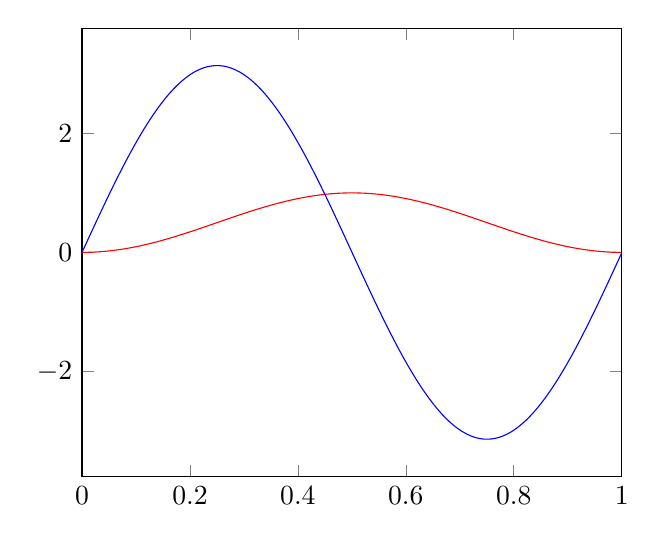
\begin{tikzpicture}
				\begin{axis}[
				clip=false,
				xmin=0,xmax=1,
				%axis lines=left,
				%axis x line=middle,
				%axis y line=left,
				]
				\addplot[domain=0:1,samples=200,red]{sin(3.14*deg(x))^2}node[right,pos=0.9]{};
				\addplot[domain=0:1,samples=200,blue]{6.28*sin(3.14*deg(x))*cos(3.14*deg(x))}node[right,pos=0.9]{};
				\end{axis}
			\end{tikzpicture}
			}
		\end{minipage}
	\end{frame}
	\begin{frame}{T-coercive elliptic problems}
	$\newline$
	\begin{definition}[T-coercivity]
		We call a sesquilinear form $\mathcal{A}(\cdot,\cdot)$ \textbf{T-coercive} on $X$ if there exists a bijective operator $T \in L(X)$ and a constant $\alpha > 0$ s.t.
		\begin{equation*}
		\mathcal{A}(Tu,u) \ge \alpha \Vert u \Vert^2_X \qquad \forall u \in X.
		\end{equation*}
	\end{definition}
	\begin{theorem}<2->[Ciarlet\footnotemark]
		If $\mathcal{A}(\cdot,\cdot)$ is T-coercive on $X$, then the corresponding variational problem is well-posed.
	\end{theorem}
	\visible<2->{
	\begin{enumerate}
		\item[\tiny 1.] \scriptsize see e.g., P. Ciarlet Jr., "T-coercivity: Application to the discretization of Helmholtz-like problems", 2012.
	\end{enumerate}
	}
	\end{frame}
	\begin{frame}{Discrete T-coercivity}
	$\newline$
	\begin{itemize}
		\item<1->[\oxarrow] T-coercivity is a \textbf{sufficient and necessary} condition for well-posedness of the weak formulation.
		\item<2->[\oxarrow] T-coercivity is \textbf{\color{red}not} automatically inherited onto the discrete level.
		\item<3->[\oxarrow] T-coercivity, at the discrete level, is a equivalent to \textbf{uniform inf-sup stability}, i.e.
		\begin{equation*}
		\inf_{v_h \in X_h} \sup_{w_h \in X_h} \frac{\vert a_h(v_h,w_h) \vert}{\Vert v_h \Vert_X \Vert w_h \Vert_X} \ge \beta > 0,
		\end{equation*}
		which guarantees the \textbf{well-posedness} of the discrete problem.
	\end{itemize}
	\end{frame}
	\begin{frame}{Compact Eigenvalue problems}
		\vspace{0.7cm}
		Considering the eigenvalue problem, find $(\lambda,P)\in \mathbb{R}\times H^1_0(\Omega)$ such that
		\begin{equation*}
			(\nabla P, \nabla Q)_{L^2} = \lambda (P,Q)_{L^2} \quad \forall Q \in H^1_0(\Omega).
		\end{equation*}
		\visible<2->{
		We can rewrite this as an eigenvalue problem associated with an operator $\mathcal{S}:H^1_0(\Omega)\to H^1_0(\Omega)$, i.e. find $(\lambda,P)\in \mathbb{R}\times H^1_0(\Omega)$ such that
		\begin{equation*}
			(\nabla \mathcal{S}f,\nabla Q) = \lambda (f,Q) \quad \forall Q \in H^1_0(\Omega).
		\end{equation*}}
		\vspace{-0.5cm}
		\visible<3->{
		\begin{block}{Elliptic regularity}
			Via elliptic regularity theory, we know that the operator $\mathcal{S}$ is compact.
			In fact, by Rellich-Kondrachov we know that $H^2(\Omega)\subset\!\subset H^1_0(\Omega)$.
		\end{block}}
	\end{frame}
	\begin{frame}{Hilbert basis}
		$\newline$
		\begin{itemize}
			\item<1->[\oxarrow] Let $(\lambda^{(i)},\Phi^{(i)})_{i\in\mathbb{N}}$ be the eigenpairs of the operator $\mathcal{S}$.
			\item<2->[\oxarrow] The eigenfunctions $(\Phi^{(i)})_{i\in\mathbb{N}}$ form a \textbf{Hilbert basis} of $H^1_0(\Omega)$.
			\item<3->[\oxarrow] We expand any $\Phi^{(i)}\in H^1_0(\Omega)$ as $P = \sum_{i\in\mathbb{N}} \Phi^{(i)}( P,\Phi^{(i)})_{H^1}$.
			\item<4->[\oxarrow] We will adopt the convection that the $\norm{\Phi^{(i)}}_{H^1}$ is unitary.
		\end{itemize}
		\visible<5->{\begin{block}{Spectral decomposition}
			$S$ is a compact operator on $H^1_0(\Omega)$, hence the eigenvalues $\lambda^{(i)}$ are \textbf{discrete} and \textbf{tend to zero}.
			Furthermore, the eigenfunctions $P^{(i)}$ form a \textbf{Hilbert basis} of $H^1_0(\Omega)$.
		\end{block}}
	\end{frame}

	\begin{frame}{T-coercivity of the Helmholtz problem}
	\vspace{1.2cm}
	\quad \oxarrow \; $\lVert \Phi^{(i)} \lVert_{H^1} = 1$ implies $\lVert \Phi^{(i)} \lVert_{L^2} = (1+\lambda^{(i)})^{-1/2}$. \\
	\vspace{-0.5cm}
	\visible<2->{
	\begin{align*}
		\mathcal{A}(P,P) &= (\nabla P,\nabla P)_{L^2} -k^2 (P,P)_{L^2(\Omega)}\\
		&= \sum_{i\in \N} P^{(i)} (\nabla \Phi^{(i)}, \nabla P)_{L^2} - k^2 P^{(i)} (\Phi^{(i)},P)_{L^2} \\
		&= \sum_{i\in \N} \lambda^{(i)} P^{(i)} (\Phi^{(i)},P)_{L^2} - k^2 P^{(i)} (\Phi^{(i)},P)_{L^2} \\
		&= \sum_{i\in \N} \lambda^{(i)} \lvert P^{(i)} \lvert^2 (\Phi^{(i)},\Phi^{(i)})_{L^2} - k^2 \lvert P^{(i)}\lvert^2 (\Phi^{(i)},\Phi^{(i)})_{L^2} \\
		&=\sum_{i \in \mathbb{N}} \left( \frac{\lambda^{(i)} - k^2}{1-\lambda^{(i)}} \right) \lvert P^{(i)}\lvert^2
	\end{align*}
	}
	\end{frame}

	\begin{frame}{T-coercivity of the Helmholtz problem}
	$\newline$
	\visible<1->{Suppose $\exists i_{\ast}$ s.t. $\lambda_1 < \dots < \lambda_{i_{\ast}} < k^2 < \lambda_{i_{\ast} + 1} < ...$}
	$\newline$
	$\newline$
	\visible<2->{
	We then construct $W := \text{span}_{0 \le i \le i_{\ast}} \{ \Phi^{(i)} \}$ and set $T := \operatorname{Id}_X - 2 P_{W}$, i.e. 
	\begin{equation*}
		T \Phi^{(i)} = \begin{cases}
		- \Phi^{(i)} & \text{if } i \le i_{\ast}, \\
		+ \Phi^{(i)} & \text{if } i > i_{\ast}.
		\end{cases}
	\end{equation*}}
	\begin{enumerate}
		\item <3->[\oxarrow] $T$ is bijective, since it is self-inverse, i.e. $T^2 = \operatorname{Id}_X$.
	\end{enumerate}
	\end{frame}
	\begin{frame}
	$\newline$
	$\newline$
	We notice that $\mathcal{A}(\cdot,\cdot)$ is T-coercive, provided $k^2$ not an eigenvalue $\lambda^{(i)}$, since
	\begin{equation*}
		\begin{aligned}
		\mathcal{A}(P,TP) &= \sum_{i \le i_{\ast}} \left( \frac{k^2 - \lambda^{(i)}}{1+\lambda^{(i)}} \right) (\Phi^{(i)})^2  + \sum_{i > i_{\ast}} \left( \frac{\lambda^{(i)} - k^2}{1+\lambda^{(i)}} \right) (\Phi^{(i)})^2  \\
		&\ge \alpha \sum_{i \in \mathbb{N}} \lambda^{(i)} (\Phi^{(i)})^2 = \alpha \Vert P \Vert^2_{H^1}, 
		\end{aligned}
	\end{equation*}
	where $\alpha = \min_{i \ge 0} \left\{ \left \vert \frac{\lambda^{(i)} - k^2}{1+\lambda^{(i)}} \right \vert \right\} > 0$.
	\end{frame}

	\begin{frame}{Weak T-coercivity}
	\vspace{0.5cm}
	\begin{definition}[weak T-coercivity]
		A linear operator $A \in L(X)$ is called \textbf{weakly T-coercive} if there exists a bijective operator $T \in L(X)$ and $K \in L(X)$ compact s.t. $T^*A + K$ is coercive. 
	\end{definition}
	\begin{itemize}
	\item<2->[\oxarrow] $A$ is T-coercive if $T^*A$ is bijective.
	\item<3->[\oxarrow] $A$ is weakly T-coercive if $T^*A + K$, $B$ bijective and $K$ compact.
	\end{itemize}
	
	\begin{lemma}<4->
	If $A$ is weakly T-coercive and injective, then $A$ is bijective. 
	\end{lemma}
	\end{frame}


	\begin{frame}{Robin boundary conditions}
	\vspace{0.8cm}
	Consider the Helmholtz problem with Robin boundary conditions, i.e. find $u \in H^1(\Omega)$ such that $\mathcal{A}(P,Q) = \prescript{}{H^{-1}}{\langle} f,Q \rangle_{H^1}$ $\forall Q \in X$, where
	\begin{equation*}
		\mathcal{A}(P,Q)\!:=\! \underbrace{(\nabla P, \nabla Q)_{L^2} \!- k (P,Q)_{L^2}}_{\mathcal{A}_0(P,Q)} {\color{gray!60!black} \!- ik \langle P, Q \rangle_{L^2(\partial \Omega)}}\! = (f , Q)_{L^2}.
	\end{equation*}
	\vspace{-0.5cm}
	\begin{block}<2->{Trace theorem}
		On bounded Lipschitz domains, the trace operator $\gamma_0 : H^1(\Omega) \to L^2(\partial \Omega)$ is compact. 
	\end{block}
	\begin{itemize}
		\item<3->[\oxarrow] The operator $\langle Ku, v \rangle_{H^1} := - i k \langle \gamma_0 u, \gamma_0 v \rangle_{L^2(\partial \Omega)}$ is compact. \\
		\item<4->[\oxarrow] $A$ is weakly T-coercive (injectivity can also be shown)
	\end{itemize}
	\end{frame}
	 
	\begin{frame}{Schatz argument}
	\vspace{0.8cm}
	We begin observing that the sesquilinear form $\mathcal{A}_0$ satisfies the \textit{G\aa rding inequality}, i.e.
	\vspace{-0.3cm }
	\begin{equation*}
		\mathcal{G}\norm{P-P_h}_{H^1_k}^2 \leq Re\left\{\mathcal{A}_0(P-P_h,P-Q_h)\right\} + k^2\norm{P-P_h}_{L^2}^2,
	\vspace{-0.5cm }
	\end{equation*}
	where we have introduced the norm $\norm{P}_{H^1_k}^2 \!:=\!\norm{\nabla P}_{L^2}^2 \!+\! k^2\norm{P}_{L^2}^2$.
	\visible<2->{
		\begin{block}{Aubin-Nitsche duality trick}
			The following bound holds,
			\begin{equation*}
				\norm{P-P_h}_{L^2} \leq M^2\psi(X_h)\norm{P-P_h}_{H^1_k},
			\end{equation*}
			where $\psi(X_h):=\underset{g\in L^2(\Omega)}{\sup}\underset{Q_h\in X_h}{\inf}\frac{\norm{g-Q_h}_{H^1_k}}{\norm{g}_{L^2}}$.
		\end{block}
	}
	\end{frame}
	\begin{frame}{Schatz argument}
		\vspace{1cm}
		Combining the G\aa rding inequality with the Aubin-Nitsche duality trick, we obtain
		\begin{equation*}
				\mathcal{G} \norm{P-P_h}_{H^1_k}^2 \leq M \norm{P-Q_h}_{H^1_k}\norm{P-P_h}_{H^1_k} + M^2k^2 \psi(X_h)^2 \norm{P-P_h}_{H^1_k}^2.
		\end{equation*}
		\visible<2->{
			Imposing the following condition on $\psi(X_h)$,
			\begin{equation}
				\psi(X_h) \leq \left(\frac{\mathcal{G}}{2k^2M^2}\right)^{\frac{1}{2}},
			\end{equation}
			we obtain the following error bound:
			\begin{equation}
				\mathcal{G}\norm{P-P_h}_{H^1_k} \leq 2M\underset{Q_h\in X_h}{\inf}\norm{P-Q_h}_{H^1_k}.
			\end{equation}
		}
	\end{frame}	
	\begin{frame}{Schatz argument}
		\vspace{1cm}
		Using \textit{Bramble-Hilbert lemma}, we can bound $\psi(X_h)$ as
		\begin{equation*}
			\psi (X_h) \leq C_\mathcal{I} h \norm{Z}_{H^2(\Omega)} \leq \left(\frac{\mathcal{G}}{2k^2M^2}\right)^{\frac{1}{2}}.
		\end{equation*}
		\vspace{-0.5cm}
		\visible<2->{
			\begin{block}{Frequency regularity estimates}
				The following regularity estimate holds $\norm{P}_{H^2}\!\leq\! (1\!+\!kC_\Omega)\norm{g}_{L^2}$, for $P\in H^2(\Omega)$ such that $-\Delta P = g$.
			\end{block}
		}
		\visible<3->{
			Combining the previous estimates we obtain,
			\vspace{-0.3cm}
			\begin{equation*}
				h \lesssim C_\mathcal{I} \left(\frac{\mathcal{G}}{2k^2M^2}\right)^{\frac{1}{2}}(1+kC_\Omega)^{-1}\sim k^{-2}.	
			\end{equation*}
		}
	\end{frame}
	\begin{frame}{Discrete T-coercivity}
	\vspace{0.4cm}
	\begin{definition}
		We call a family of sesquilinear forms $(\mathcal{A}_h)_{h>0}$ on $X_h$ \textbf{\color{red}uniformly} T$_h$-coercive, if there exists bijective operators $T_h : X_h \to X_h$ and $\alpha > 0$ independent of $h$ s.t.
		\vspace{-0.3cm}
		\begin{equation*}
		\mathcal{A}_h(P_h,T_h P_h) \ge \alpha \Vert P_h \Vert^2_{X} \qquad \forall P_h \in X_h.
		\end{equation*}
	\end{definition}
	\visible<2->{
	\oxarrow \ \normalsize If $\mathcal{A}_h$ is uniformly T$_h$-coercive, then the discrete problem is stable and quasi-optimal $\Vert P - P_h \Vert_{X} \lesssim \inf_{P_h \in X_h} \Vert P - Q_h \Vert_{X}.$}
	\\
	\visible<3->{
	\textbf{Provided} it is usually enough to show that 
	\vspace{-0.2cm}
	\begin{equation*}
		\lim_{h \to 0} \Vert T - T_h \Vert_{X} = 0,
	\end{equation*}
	but this is an asymptotic result not explicit about $h$. 
	}
	\end{frame}

	\begin{frame}{Discrete weak T-coercivity}
	\vspace{0.7cm}
	\begin{theorem}
		Let $A = B + K$, where $B$ is bijective and $K$ compact and suppose that $\operatorname{ker}(A) = \{ 0 \}$. If there exists a family of bijective operators $T_h \in \mathcal{L}(X_h)$ s.t. $B$ is \textbf{\color{red} uniformly T$_h$-coercive} on $X_h$, then there exists $h_0 > 0$ s.t. $A$ is \textbf{\color{red} uniformly T$_h$-coercive} on $X_h$ for $h < h_0$.
	\end{theorem}
	$\newline$
	\oxarrow \ \normalsize If $A$ is weakly coercive and injective, and $(T^{\ast})^{-1} B$ is uniformly T$_h$-coercive, then the discrete problem is stable and quasi-optimal
	\begin{equation*}
		\Vert P - P_h \Vert_{X} \lesssim \inf_{Q_h \in X_h} \Vert P - Q_h \Vert_{X}.
	\end{equation*}
	\end{frame}

	\begin{frame}{Discrete Helmholtz}
	\vspace{1cm}
	Find $P_h \in X_h$ such that for any $P_h\in X_h$ the following holds,
	\begin{equation*}
		\mathcal{A}(P_h,Q_h)\!:=\! \underbrace{(\nabla P_h, \nabla Q_h)_{L^2} \!- k (P_h,Q_h)_{L^2}}_{=: \mathcal{A}_0(P_h,Q_h)} {\color{gray!60!black} \!- ik \langle P_h, Q_h \rangle_{L^2(\partial \Omega)}}\! = (f , Q_h)_{L^2}.
	\end{equation*}
	\visible<2->{
	\Large \oxarrow \ \normalsize Only have to show that $\mathcal{A}_0$ is uniformly T$_h$-coercive. \\
	Define $T_h : X_h \to X_h$ through 
	\begin{equation*}
		T_h e_h^{(i)} := \begin{cases}
		- e_h^{(i)} & \text{if } i \le i_{\ast}, \\
		+ e_h^{(i)} & \text{if } i > i_{\ast}.
		\end{cases}
	\end{equation*}}
	\end{frame}
	\begin{frame}{Discrete T-coercivity of $\mathcal{A}_0$}
	\vspace{0.5cm}
	Following the same steps as before, we can expand $P_h$ in terms of the eigenfunctions of $\mathcal{S}: X_h\to X_h$, i.e. $P_h = \sum_{i \in \mathbb{N}} P_h^{(i)} \Phi_h^{(i)}$.
	\begin{equation*}
		\mathcal{A}_0(P_h,T_h P_h) := \sum_{i \le i_{\ast}} \left( \frac{k - \lambda_h^{(i)}}{1+\lambda_h^{(i)}} \right) (P_h^{(i)})^2  + \sum_{i > i_{\ast}} \left( \frac{\lambda_h^{(i)} - k}{1+\lambda_h^{(i)}} \right) (P_h^{(i)})^2.
	\end{equation*}
	\begin{itemize}
		\item<2->[\oxarrow] $\mathcal{A}_0$ is uniformly T$_h$-coercive if and only if $\lambda_h^{(i_{\ast})} < k^2$.
		\item<3->[\oxarrow] This is equivalent to ensure that $\lambda_h^{(i_{\ast})} - \lambda^{(i_{\ast})} < k^2 - \lambda^{(i_{\ast})}$ \\
	\end{itemize}
	\end{frame}

	\begin{frame}{Discrete T-coercivity of $\mathcal{A}_0$}
		\vspace{0.7cm}
		\begin{figure}
			\centering
			\only<1>{
				\includegraphics[scale=0.5]{Figures/convergence_k_10_k_12.png}
				\vspace{-0.3cm}
				\caption{
					$L^2$-error of the approximation of the Helmholtz problem with Dirichlet boundary conditions against a computed reference solution.
					$\newline$
					The vertical lines indicate when $\lambda_h^{(i_{\ast})} < k^2$.
				}
			}
			\only<2>{
				\includegraphics[scale=0.5]{Figures/convergence_k_15_k_20.png}
				\vspace{0.1cm}
				\caption{
					$L^2$-error of the approximation of the Helmholtz problem with Dirichlet boundary conditions against a computed reference solution.
					$\newline$
					The vertical lines indicate when $\lambda_h^{(i_{\ast})} < k^2$.
				}
			}
		\end{figure}
	\end{frame}

	\begin{frame}{Eigenvalue estimates}
	\vspace{1cm}
	With classical eigenvalue estimates, we get 
	\begin{equation*}
		\lambda_h^{(i_{\ast})} - \lambda^{(i_{\ast})} \le \lambda^{(i_\ast)} 4 \sqrt{i_\ast} C_{\Omega,X} C_{\mathcal{I}} h^2,
	\end{equation*}
	where the constant $C_{\Omega,X}$ and $C_{\mathcal{I}}$ are defined as follows:
	\begin{itemize}
		\item<2->[\oxarrow] $C_{\Omega,X} = C_P/\kappa$ where $C_P$ is the Poincaré constant and $\alpha$ is the coercivity constant of $-\Delta$.
		\item<3->[\oxarrow] $C_{\mathcal{I}}$ is the interpolation constant. 
	\end{itemize}
	\visible<4->{
	So to have uniform T$_h$-coercivity, we want to ensure that  
	\begin{equation*}
		h^2 < \frac{k^2 - \lambda^{(i_{\ast})}}{ 4 \sqrt{i_\ast} \lambda^{(i_\ast)} C_{\Omega,X} C_{\mathcal{I}}}.
	\end{equation*}
	}
	\end{frame}

	\begin{frame}{Quasi-optimality of $\mathcal{A}_0$}
	\vspace{0.7cm}
	\begin{minipage}{0.6\textwidth}
	\begin{theorem}
		The bilinear form $\mathcal{A}_0$ is uniformly T$_h$-coercive on $X_h$, if $h$ is chosen such that
		\vspace{-0.3cm}
		\begin{equation*}
		h^{2} < \frac{k^2 - \lambda^{(i_{\ast})}}{ 4 \sqrt{i_\ast} \lambda^{(i_\ast)} C_{\Omega,X} C_{\mathcal{I}}}.
		\end{equation*}
	\end{theorem}
	\end{minipage}
	\,
	\begin{minipage}{0.3\textwidth}
	\begin{figure}
		\visible<2->{
		\centering
		\vspace{1.cm}
		\includegraphics[scale=0.4]{Figures/eigenvalue_estimates.png}
		}
	\end{figure}
	\end{minipage}
	\vspace{0.5cm}
	\begin{itemize}
		\item<3->[\oxarrow] This guarantees that the discrete problem is quasi-optimal provided $h$ is small enough.
	\end{itemize}
	\end{frame}

	\begin{frame}{Adaptive scheme}
	\vspace{1cm}
	Construct the mesh, with the minimal number of elements, that guarantees the quasi-optimality of the Helmholtz problem:
	\begin{enumerate}
		\item<2->[\oxarrow] \textbf{Determine $i_{\ast}$:} either we know the eigenvalues, or we have to approximate them well enough (but we can choose any method we like to do this). 
		\item<3->[\oxarrow] \textbf{Solving the Laplace eigenvalue problem adaptively:} Solve the Laplace eigenvalue problem on a sequence of refined meshes and check whether $k^2 - \lambda_h^{(i_{\ast})} < 0$. If yes, we can stop because $h$ is small enough s.t. we have uniform T$_h$-coercivity. (needs to use the same discretization as for Helmholtz)
		\item<4->[\oxarrow] \textbf{Solve the Helmholtz problem.}
	\end{enumerate}
	\end{frame}
	\begin{frame}{Adpative scheme: numerical examples}
		\vspace{0.7cm}
		\only<1>{
		\begin{figure}
			\centering
			\includegraphics[scale=0.6]{Figures/pitch_uniform_step_1.png}
		\end{figure}
		}
		\only<2>{
		\begin{figure}
			\centering
			\includegraphics[scale=0.6]{Figures/pitch_uniform_step_2.png}
		\end{figure}
		}
		\only<3>{
		\begin{figure}
			\centering
			\includegraphics[scale=0.6]{Figures/pitch_uniform_step_3.png}
		\end{figure}
		}
		\only<4>{
		\begin{figure}
			\centering
			\includegraphics[scale=0.6]{Figures/pitch_uniform_step_4.png}
		\end{figure}
		}
	\end{frame}
	\begin{frame}{Adaptive$^2$ scheme}
	\begin{itemize}
		\item[\oxarrow] In the adaptive scheme, we use a \textbf{Babuška--Rheinboldt} estimator to adaptively refine the mesh.
		\item[\oxarrow] The main idea is to use the \textbf{Babuška--Rheinboldt} estimator not one the desired solution or on a specific eigenfunction, but rather on the first $i_{\ast}+\ell$ eigenfunctions, i.e.
		\begin{equation*}
			\eta_K\! =\! i_{\ast}^{-1}\!\!\sum_{i = 1}^{i_{\ast}+\ell}\! h^2_K \Vert \Delta e_h^{(i)} \!+\!\lambda_h^{(i)} e_h^{(i)} \Vert^2_{L^2(K)} \!+\! \frac{h_K}{2} \Vert \nabla e_h^{(i)}\! \cdot n \Vert^2_{L^2(\partial K \setminus \partial \Omega)}.
		\end{equation*}
		\item[\oxarrow] We then refine the mesh in the elements where the indicator is larger. We can also adapt a \textbf{D\"orfler marking} strategy.
	\end{itemize} 
	\end{frame}
	\begin{frame}{Adpative$^2$ scheme: numerical examples}
		\vspace{0.7cm}
		\only<1>{
		\begin{figure}
			\centering
			\includegraphics[scale=0.6]{Figures/pitch_adpt_step_1.png}
		\end{figure}
		}
		\only<2>{
		\begin{figure}
			\centering
			\includegraphics[scale=0.6]{Figures/pitch_adpt_step_2.png}
		\end{figure}
		}
		\only<3>{
		\begin{figure}
			\centering
			\includegraphics[scale=0.6]{Figures/pitch_adpt_step_3.png}
		\end{figure}
		}
		\only<4>{
		\begin{figure}
			\centering
			\includegraphics[scale=0.6]{Figures/pitch_adpt_step_4.png}
		\end{figure}
		}
	\end{frame}
\end{document}


\pgfdeclareimage[width=\paperwidth]{titlebackground}{Images/title-slide-background.png}
\setbeamerfont{subtitle}{size=\tiny}
\setbeamertemplate{endpage}{
	\begin{picture}(0,0)
		\scalebox{1.01}{
		\put(-28.5,-163){%
			\pgfuseimage{titlebackground}
		}
		}
		\put(0,-115){%
			\begin{minipage}[b][4.5cm][t]{0.5\textwidth}
				\color{white}
				\usebeamerfont{title}
				{\textbf{Thank Your} \\ \textbf{For You Attention !}}
			\end{minipage}
		}
	\end{picture}
}
\setbeamertemplate{title page}{
	\begin{picture}(0,0)
		\scalebox{1.01}{
			\put(-28.5,-163){%
				\pgfuseimage{titlebackground}
			}
		}
		\put(0,-60){%
			\begin{minipage}[b][4.5cm][t]{0.7\textwidth}
				\color{white}
				\usebeamerfont{title}
				{\inserttitle\\[0.9cm]}
				\usebeamerfont{subtitle}
				{\insertauthor\par}
				{\insertinstitute\\[0.3cm]}
				{\insertdate}
			\end{minipage}
		}
	\end{picture}
}


%% General slide formatting %%

\definecolor{oxfordblue}{RGB}{4,30,66}
\definecolor{oxfordred}{RGB}{207,48,42}

\pgfdeclareimage[width=0.9cm]{oxfordlogo}{Images/oxford-logo.png}
\pgfdeclareimage[width=1cm]{mathslogo}{Images/mathematics-logo.png}
\pgfdeclareimage[width=1.2cm]{ngslogo}{Images/ngs-logo.png}
\pgfdeclareimage[width=1.2cm]{petsclogo}{Images/petsc-logo.png}
\pgfdeclareimage[width=1.2cm]{firedrakelogo}{Images/firedrake-logo.png}

\setbeamertemplate{headline}
{%
	\begin{picture}(0,0)
		\put(314,-50){%
			\pgfuseimage{oxfordlogo}
		}
		\put(20,-55){%
			\rule{320pt}{0.4pt}
		}
	\end{picture}
}
\def\ngshead{
	\begin{picture}(0,0)
		\put(278,0){%
			\pgfuseimage{ngslogo}
		}
		\put(-8,-5){%
			\rule{325pt}{0.4pt}
		}
	\end{picture}
}
\def\petschead{
	\begin{picture}(0,0)
		\put(278,0){%
			\pgfuseimage{petsclogo}
		}
		\put(-8,-5){%
			\rule{325pt}{0.4pt}
		}
	\end{picture}
}
\def\firedrakehead{
	\begin{picture}(0,0)
		\put(278,0){%
			\pgfuseimage{firedrakelogo}
		}
		\put(-8,-5){%
			\rule{325pt}{0.4pt}
		}
	\end{picture}
}
\setbeamertemplate{frametitle}
{%
	\begin{picture}(0,0)
		\put(-8,-20){%
			\normalsize\textbf{\color{oxfordblue}\insertframetitle}
		}
		\put(-8,-32){%
			\normalsize\textbf{\color{oxfordblue}\insertframesubtitle}
		}
	\end{picture}
}

\setbeamertemplate{footline}
{%
	\begin{picture}(0,0)
		\put(20,30){%
			\rule{320pt}{0.4pt}
		}
		\put(20,14){%
			\pgfuseimage{mathslogo}
		}
		\put(100,14){%
			\color{oxfordblue}\insertshortdate
		}
		\put(160,14){%
			\color{oxfordblue}\insertshorttitle
		}
		\put(337,14){%
			\color{oxfordblue}\insertframenumber
		}
	\end{picture}%
}
\def\footer{
	\begin{picture}(0,0)
		\put(-308,-75){%
			\rule{325pt}{0.4pt}
		}
		\put(-308,-91){%
			\pgfuseimage{mathslogo}
		}
		\put(-228,-91){%
			\color{oxfordblue}\tiny\insertshortdate
		}
		\put(-168,-91){%
			\color{oxfordblue}\tiny\insertshorttitle
		}
		\put(9,-91){%
			\color{oxfordblue}\tiny\insertframenumber
		}
	\end{picture}
}

\setbeamercolor{block title}{bg=oxfordblue!30,fg=black}
\setbeamercolor{palette primary}{bg=oxfordblue,fg=white}

\definecolor{codegreen}{rgb}{0,0.6,0}
\definecolor{codegray}{rgb}{0.5,0.5,0.5}
\definecolor{codepurple}{rgb}{0.58,0,0.82}
\definecolor{backcolour}{rgb}{0.95,0.95,0.92}

\lstdefinestyle{mystyle}{
	%backgroundcolor=\color{backcolour},   
	commentstyle=\color{codegray},
	keywordstyle=\color{oxfordblue},
	numberstyle=\tiny\color{codegray},
	stringstyle=\color{codegreen},
	basicstyle=\ttfamily\footnotesize,
	breakatwhitespace=false,         
	breaklines=true,                 
	captionpos=b,                    
	keepspaces=true,                 
	numbers=left,                    
	numbersep=5pt,                  
	showspaces=false,                
	showstringspaces=false,
	showtabs=false,                  
	tabsize=2
}
\AtBeginSection[]{
  \begin{frame}
  \vfill
  \centering
  \begin{beamercolorbox}[sep=8pt,center,shadow=true,rounded=true]{title}
    \usebeamerfont{title}\insertsectionhead\par%
  \end{beamercolorbox}
  \vfill
  \end{frame}
}

\lstset{style=mystyle}

%Specific macros
\newcommand{\oxarrow}{\color{oxfordblue}$\blacktriangleright$}
\newcommand{\N}{\mathbb{N}}

%% Information (author, title, etc.) %%
\title[Helmholtz]{Quasi-optimality of FEMs for the Helmholtz equation}
\author%
{%
	\sc{T.~van~Beeck$^\dag$}, \underline{\sc{U.~Zerbinati}}$^*$\\
}
\institute%
{%
	* \textit{Mathematical Institute}\\
	\;\textit{University of Oxford}\\
	$\newline$
	$\dag$ \textit{Institute for Numerical and Applied Mathematics}\\
	\;\textit{University of G\"ottingen}\\	
}

\date[\textbf{PYSANUM}]{} 



%% Content of slides %%

\begin{document}
	\begin{frame}[plain]
		\titlepage
	\end{frame}

	\begin{frame}{The wave equation}
		\visible<1->{The \textbf{wave equation} is a second-order linear partial differential equation for the description of waves.}
		$\newline$
		$\newline$
		\visible<2->{In particular, it describes the evolution of an \textbf{excess pressure} $p_\delta$ in a medium with speed of sound $c$.}
		\visible<3->{
		\begin{equation}
			\begin{aligned}
				\partial_t^2 p_\delta - c^2\Delta p_\delta &= f \quad &\text{in } \;\;\;\Omega \times (0,T), \\
				p_\delta &= 0 \quad &\text{on } \partial \Omega \times (0,T), \\
				p_\delta(\cdot,0) &= p_0(\cdot), \quad & \partial_t p_\delta(\cdot,0) = \dot{p}_0(\cdot).
			\end{aligned}
		\end{equation}}
	\end{frame}

	\begin{frame}{Time harmonic solutions of the wave equation}
		$\newline$
		\visible<1->{The \textbf{time harmonic solutions} of the wave equation are of the form}
		\begin{equation}
			p^{(\delta)}(\cdot,t) = \Re\left\{ P(\cdot) e^{-i\omega t} \right\},
		\end{equation}
		\visible<1->{where $P:\Omega\to \mathbb{C}$ and $\omega$ is the \textbf{angular frequency}.}
		$\newline$
		\visible<2->{Substituting this ansatz into the wave equation, we obtain the \textbf{Helmholtz equation}
		\begin{equation}
			\begin{aligned}
				- \Delta P - k^2 P &= F \quad &\text{in } \;\;\;\Omega, \\
				u &= 0 \quad &\text{on } \partial \Omega,
			\end{aligned}
		\end{equation}}
		\visible<2->{where $k = \omega/c$ is the \textbf{wave number} and $F = \Re\left\{f(\cdot,t)e^{-i\omega t}\right\}$.}
	\end{frame}
	\begin{frame}{The weak formulation}
		$\newline$
		\visible<1->{The \textbf{weak formulation} of the Helmholtz equation is to find $u \in H^1_0(\Omega)$ such that
		\begin{equation}
			\begin{aligned}
				(\nabla P, \nabla Q)_{L^2} - k^2 (P,Q)_{L^2} &= \prescript{}{H^{-1}}{\langle} F,Q \rangle_{H^1_0} \quad \forall Q \in H^1_0(\Omega),
			\end{aligned}
		\end{equation}
		where $(\cdot,\cdot)_{L^2}$ denotes the $L^2$ inner product.}
		$\newline$
		$\newline$
		\visible<2->{The weak formulation of the Helmholtz equation is \textbf{elliptic}, hence we can make use of \textbf{elliptic regularity theory}.}
		$\newline$
		$\newline$
		\visible<3->{The Helmholtz problem is \textbf{ill-posed} if $k^2$ is an eigenvalue of the Laplacian, in the sense that the solution $P$ is not uniquely determined by the data $F$.}
	\end{frame}
	\begin{frame}{Finite element discretization}
		\vspace{0.8cm}
		\visible<1->{The \textbf{finite element discretization} of the Helmholtz equation is to find $u_h \in X_h$ such that
		\begin{equation}
			\begin{aligned}
				(\nabla P_h, \nabla Q_h)_{L^2} - k^2 (P_h,Q_h)_{L^2} &= (F,Q_h)_{L^2} \quad \forall Q_h \in X_h,
			\end{aligned}
		\end{equation}
		where $X_h \subset H^1_0(\Omega)$ is a finite-dimensional subspace.}
		\begin{itemize}
			\item<2->[\oxarrow] We discretize the domain $\Omega$ into a mesh of elements $\{\mathcal{T}_h\}_{h>0}$.
			\item<3->[\oxarrow] We choose as $X_h$ the space of piecewise linear polynomial functions on the mesh, i.e.
			\begin{equation*}
				X_h := \{ v \in L^2(\Omega) : v \vert_{\tau} \in \mathcal{P}^1(\tau) \ \forall \tau \in T_h \} \cap H^1_0(\Omega) \subset H^1_0(\Omega).
			\end{equation*}
			\item<4->[\oxarrow] We obtain a \textbf{linear system} of the form $\underline{\underline{\mathcal{A}}} \,\underline{P}_h = \underline{F}$.
		\end{itemize}	
	\end{frame}
	\begin{frame}{A motivating example}
		$\newline$
		$\newline$
		\begin{equation}
			P(\cdot) = \sin(\pi \omega \cdot), \qquad \omega = 16
		\end{equation}
		$\newline$
		\only<2>{
			\begin{minipage}{0.3\textwidth}
				\begin{figure}
					\centering
					\includegraphics[scale=0.3]{Figures/proj_N_6_omega_16.png}
					\caption{$L^2$ projection}
				\end{figure}
			\end{minipage}
			\begin{minipage}{0.3\textwidth}
				\begin{figure}
					\centering
					\includegraphics[scale=0.3]{Figures/poisson_N_6_omega_16.png}
					\caption{$k=0$}
				\end{figure}
			\end{minipage}
			\begin{minipage}{0.3\textwidth}
				\begin{figure}
					\centering
					\includegraphics[scale=0.3]{Figures/helmholtz_N_6_omega_16.png}
					\caption{$k=256$}
				\end{figure}
			\end{minipage}
		}
		\only<3>{
			\begin{minipage}{0.3\textwidth}
				\begin{figure}
					\centering
					\includegraphics[scale=0.3]{Figures/proj_N_24_omega_16.png}
					\caption{$L^2$ projection}
				\end{figure}
			\end{minipage}
			\begin{minipage}{0.3\textwidth}
				\begin{figure}
					\centering
					\includegraphics[scale=0.3]{Figures/poisson_N_24_omega_16.png}
					\caption{$k=0$}
				\end{figure}
			\end{minipage}
			\begin{minipage}{0.3\textwidth}
				\begin{figure}
					\centering
					\includegraphics[scale=0.3]{Figures/helmholtz_N_24_omega_16.png}
					\caption{$k=256$}
				\end{figure}
			\end{minipage}
		}
		\only<4>{
			\begin{minipage}{0.3\textwidth}
				\begin{figure}
					\centering
					\includegraphics[scale=0.3]{Figures/proj_N_48_omega_16.png}
					\caption{$L^2$ projection}
				\end{figure}
			\end{minipage}
			\begin{minipage}{0.3\textwidth}
				\begin{figure}
					\centering
					\includegraphics[scale=0.3]{Figures/poisson_N_48_omega_16.png}
					\caption{$k=0$}
				\end{figure}
			\end{minipage}
			\begin{minipage}{0.3\textwidth}
				\begin{figure}
					\centering
					\includegraphics[scale=0.3]{Figures/helmholtz_N_48_omega_16.png}
					\caption{$k=256$}
				\end{figure}
			\end{minipage}
		}
	\end{frame}

	\begin{frame}{Coercive elliptic problems}
	\vspace{0.8cm}
	\begin{definition}<1->[Coercivity]
		We call a sesquilinear form $\mathcal{A}:X\times X\to \mathbb{C}$ \textbf{coercive} on $X$ if there exists a constant $\alpha > 0$ such that
		\begin{equation*}
		\mathcal{A}(P,P) \ge \alpha \Vert P \Vert^2_X \qquad \forall P \in X. 
		\end{equation*}
	\end{definition}
	\begin{theorem}<2->[Lax-Milgram]
		If $\mathcal{A}:X\times X\to\mathbb{C}$ is coercive on $X$, then the variational problem 
		\begin{equation*}
		\text{find } P \in X \text{ such that } \mathcal{A}(P,Q) = \prescript{}{X'}{\langle} f,Q\rangle_{X} \quad \forall Q \in X
		\end{equation*}
		is \textbf{well-posed} for all $f \in X'$.
	\end{theorem}
	\end{frame}
	\begin{frame}{Discrete coercive problems}
		$\newline$
		\begin{itemize}
			\item [\oxarrow] Via Lax-Milgram, we also know that the discrete problem is well-posed if the bilinear form is coercive.
		\end{itemize}
		\begin{block}<2->{Cea's lemma}
			Let $\mathcal{A}:X \times X\to\mathbb{C}$ be coercive on $X$ and let $P\in X$ be the solution of the continuous variational problem. Then the solution $P_h\in X_h$ of the discrete variational problem satisfies
			\begin{equation*}
			\Vert P-P_h \Vert_X \le \frac{M}{\alpha} \inf_{Q_h \in X_h} \Vert P - Q_h \Vert_X,
			\end{equation*}
			where $M$ is the continuity constant of $\mathcal{A}$. 

		\end{block}
	\end{frame}
	\begin{frame}{Lack of coercivity of the Helmholtz problem}
		$\newline$
		Consider the function $P(x) = \sin(\pi \omega x)$.
		\begin{minipage}{0.6\textwidth}
		\begin{align}
		&\norm{P}^2_{L^2\left([0,1]\right)}\! =\! \int_0^1 \sin^2(\pi \omega x) = \frac{1}{2}\\
		&\norm{P'}^2_{L^2\left([0,1]\right)}\! =\! \int_0^1 2\pi\sin(\pi \omega x)\cos(\pi\omega x)
		\end{align}
		notice that the last integral vanishes for $\omega \in \mathbb{N}$, on the interval $[0,1]$.
		\end{minipage}
		\begin{minipage}{0.35\textwidth}
			\scalebox{0.5}[0.5]{
			  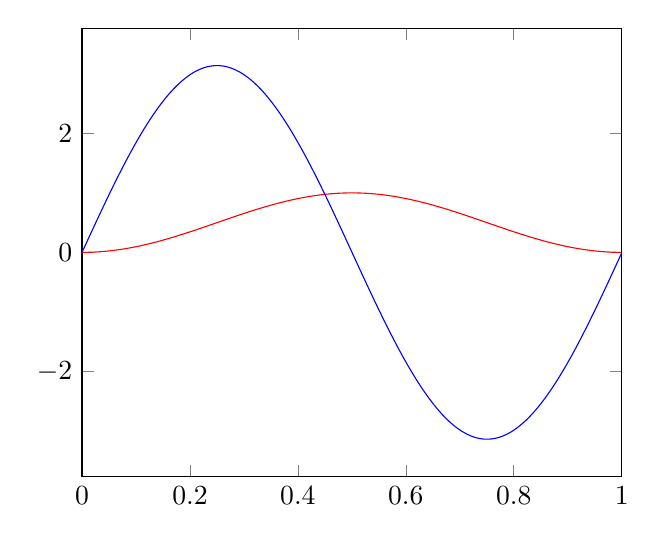
\begin{tikzpicture}
				\begin{axis}[
				clip=false,
				xmin=0,xmax=1,
				%axis lines=left,
				%axis x line=middle,
				%axis y line=left,
				]
				\addplot[domain=0:1,samples=200,red]{sin(3.14*deg(x))^2}node[right,pos=0.9]{};
				\addplot[domain=0:1,samples=200,blue]{6.28*sin(3.14*deg(x))*cos(3.14*deg(x))}node[right,pos=0.9]{};
				\end{axis}
			\end{tikzpicture}
			}
		\end{minipage}
	\end{frame}
	\begin{frame}{T-coercive elliptic problems}
	$\newline$
	\begin{definition}[T-coercivity]
		We call a sesquilinear form $\mathcal{A}(\cdot,\cdot)$ \textbf{T-coercive} on $X$ if there exists a bijective operator $T \in L(X)$ and a constant $\alpha > 0$ s.t.
		\begin{equation*}
		\mathcal{A}(Tu,u) \ge \alpha \Vert u \Vert^2_X \qquad \forall u \in X.
		\end{equation*}
	\end{definition}
	\begin{theorem}<2->[Ciarlet\footnotemark]
		If $\mathcal{A}(\cdot,\cdot)$ is T-coercive on $X$, then the corresponding variational problem is well-posed.
	\end{theorem}
	\visible<2->{
	\begin{enumerate}
		\item[\tiny 1.] \scriptsize see e.g., P. Ciarlet Jr., "T-coercivity: Application to the discretization of Helmholtz-like problems", 2012.
	\end{enumerate}
	}
	\end{frame}
	\begin{frame}{Discrete T-coercivity}
	$\newline$
	\begin{itemize}
		\item<1->[\oxarrow] T-coercivity is a \textbf{sufficient and necessary} condition for well-posedness of the weak formulation.
		\item<2->[\oxarrow] T-coercivity is \textbf{\color{red}not} automatically inherited onto the discrete level.
		\item<3->[\oxarrow] T-coercivity, at the discrete level, is a equivalent to \textbf{uniform inf-sup stability}, i.e.
		\begin{equation*}
		\inf_{v_h \in X_h} \sup_{w_h \in X_h} \frac{\vert a_h(v_h,w_h) \vert}{\Vert v_h \Vert_X \Vert w_h \Vert_X} \ge \beta > 0,
		\end{equation*}
		which guarantees the \textbf{well-posedness} of the discrete problem.
	\end{itemize}
	\end{frame}
	\begin{frame}{Compact Eigenvalue problems}
		\vspace{0.7cm}
		Considering the eigenvalue problem, find $(\lambda,P)\in \mathbb{R}\times H^1_0(\Omega)$ such that
		\begin{equation*}
			(\nabla P, \nabla Q)_{L^2} = \lambda (P,Q)_{L^2} \quad \forall Q \in H^1_0(\Omega).
		\end{equation*}
		\visible<2->{
		We can rewrite this as an eigenvalue problem associated with an operator $\mathcal{S}:H^1_0(\Omega)\to H^1_0(\Omega)$, i.e. find $(\lambda,P)\in \mathbb{R}\times H^1_0(\Omega)$ such that
		\begin{equation*}
			(\nabla \mathcal{S}f,\nabla Q) = \lambda (f,Q) \quad \forall Q \in H^1_0(\Omega).
		\end{equation*}}
		\vspace{-0.5cm}
		\visible<3->{
		\begin{block}{Elliptic regularity}
			Via elliptic regularity theory, we know that the operator $\mathcal{S}$ is compact.
			In fact, by Rellich-Kondrachov we know that $H^2(\Omega)\subset\!\subset H^1_0(\Omega)$.
		\end{block}}
	\end{frame}
	\begin{frame}{Hilbert basis}
		$\newline$
		\begin{itemize}
			\item<1->[\oxarrow] Let $(\lambda^{(i)},\Phi^{(i)})_{i\in\mathbb{N}}$ be the eigenpairs of the operator $\mathcal{S}$.
			\item<2->[\oxarrow] The eigenfunctions $(\Phi^{(i)})_{i\in\mathbb{N}}$ form a \textbf{Hilbert basis} of $H^1_0(\Omega)$.
			\item<3->[\oxarrow] We expand any $\Phi^{(i)}\in H^1_0(\Omega)$ as $P = \sum_{i\in\mathbb{N}} \Phi^{(i)}( P,\Phi^{(i)})_{H^1}$.
			\item<4->[\oxarrow] We will adopt the convection that the $\norm{\Phi^{(i)}}_{H^1}$ is unitary.
		\end{itemize}
		\visible<5->{\begin{block}{Spectral decomposition}
			$S$ is a compact operator on $H^1_0(\Omega)$, hence the eigenvalues $\lambda^{(i)}$ are \textbf{discrete} and \textbf{tend to zero}.
			Furthermore, the eigenfunctions $P^{(i)}$ form a \textbf{Hilbert basis} of $H^1_0(\Omega)$.
		\end{block}}
	\end{frame}

	\begin{frame}{T-coercivity of the Helmholtz problem}
	\vspace{1.2cm}
	\quad \oxarrow \; $\lVert \Phi^{(i)} \lVert_{H^1} = 1$ implies $\lVert \Phi^{(i)} \lVert_{L^2} = (1+\lambda^{(i)})^{-1/2}$. \\
	\vspace{-0.5cm}
	\visible<2->{
	\begin{align*}
		\mathcal{A}(P,P) &= (\nabla P,\nabla P)_{L^2} -k^2 (P,P)_{L^2(\Omega)}\\
		&= \sum_{i\in \N} P^{(i)} (\nabla \Phi^{(i)}, \nabla P)_{L^2} - k^2 P^{(i)} (\Phi^{(i)},P)_{L^2} \\
		&= \sum_{i\in \N} \lambda^{(i)} P^{(i)} (\Phi^{(i)},P)_{L^2} - k^2 P^{(i)} (\Phi^{(i)},P)_{L^2} \\
		&= \sum_{i\in \N} \lambda^{(i)} \lvert P^{(i)} \lvert^2 (\Phi^{(i)},\Phi^{(i)})_{L^2} - k^2 \lvert P^{(i)}\lvert^2 (\Phi^{(i)},\Phi^{(i)})_{L^2} \\
		&=\sum_{i \in \mathbb{N}} \left( \frac{\lambda^{(i)} - k^2}{1-\lambda^{(i)}} \right) \lvert P^{(i)}\lvert^2
	\end{align*}
	}
	\end{frame}

	\begin{frame}{T-coercivity of the Helmholtz problem}
	$\newline$
	\visible<1->{Suppose $\exists i_{\ast}$ s.t. $\lambda_1 < \dots < \lambda_{i_{\ast}} < k^2 < \lambda_{i_{\ast} + 1} < ...$}
	$\newline$
	$\newline$
	\visible<2->{
	We then construct $W := \text{span}_{0 \le i \le i_{\ast}} \{ \Phi^{(i)} \}$ and set $T := \operatorname{Id}_X - 2 P_{W}$, i.e. 
	\begin{equation*}
		T \Phi^{(i)} = \begin{cases}
		- \Phi^{(i)} & \text{if } i \le i_{\ast}, \\
		+ \Phi^{(i)} & \text{if } i > i_{\ast}.
		\end{cases}
	\end{equation*}}
	\begin{enumerate}
		\item <3->[\oxarrow] $T$ is bijective, since it is self-inverse, i.e. $T^2 = \operatorname{Id}_X$.
	\end{enumerate}
	\end{frame}
	\begin{frame}
	$\newline$
	$\newline$
	We notice that $\mathcal{A}(\cdot,\cdot)$ is T-coercive, provided $k^2$ not an eigenvalue $\lambda^{(i)}$, since
	\begin{equation*}
		\begin{aligned}
		\mathcal{A}(P,TP) &= \sum_{i \le i_{\ast}} \left( \frac{k^2 - \lambda^{(i)}}{1+\lambda^{(i)}} \right) (\Phi^{(i)})^2  + \sum_{i > i_{\ast}} \left( \frac{\lambda^{(i)} - k^2}{1+\lambda^{(i)}} \right) (\Phi^{(i)})^2  \\
		&\ge \alpha \sum_{i \in \mathbb{N}} \lambda^{(i)} (\Phi^{(i)})^2 = \alpha \Vert P \Vert^2_{H^1}, 
		\end{aligned}
	\end{equation*}
	where $\alpha = \min_{i \ge 0} \left\{ \left \vert \frac{\lambda^{(i)} - k^2}{1+\lambda^{(i)}} \right \vert \right\} > 0$.
	\end{frame}

	\begin{frame}{Weak T-coercivity}
	\vspace{0.5cm}
	\begin{definition}[weak T-coercivity]
		A linear operator $A \in L(X)$ is called \textbf{weakly T-coercive} if there exists a bijective operator $T \in L(X)$ and $K \in L(X)$ compact s.t. $T^*A + K$ is coercive. 
	\end{definition}
	\begin{itemize}
	\item<2->[\oxarrow] $A$ is T-coercive if $T^*A$ is bijective.
	\item<3->[\oxarrow] $A$ is weakly T-coercive if $T^*A + K$, $B$ bijective and $K$ compact.
	\end{itemize}
	
	\begin{lemma}<4->
	If $A$ is weakly T-coercive and injective, then $A$ is bijective. 
	\end{lemma}
	\end{frame}


	\begin{frame}{Robin boundary conditions}
	\vspace{0.8cm}
	Consider the Helmholtz problem with Robin boundary conditions, i.e. find $u \in H^1(\Omega)$ such that $\mathcal{A}(P,Q) = \prescript{}{H^{-1}}{\langle} f,Q \rangle_{H^1}$ $\forall Q \in X$, where
	\begin{equation*}
		\mathcal{A}(P,Q)\!:=\! \underbrace{(\nabla P, \nabla Q)_{L^2} \!- k (P,Q)_{L^2}}_{\mathcal{A}_0(P,Q)} {\color{gray!60!black} \!- ik \langle P, Q \rangle_{L^2(\partial \Omega)}}\! = (f , Q)_{L^2}.
	\end{equation*}
	\vspace{-0.5cm}
	\begin{block}<2->{Trace theorem}
		On bounded Lipschitz domains, the trace operator $\gamma_0 : H^1(\Omega) \to L^2(\partial \Omega)$ is compact. 
	\end{block}
	\begin{itemize}
		\item<3->[\oxarrow] The operator $\langle Ku, v \rangle_{H^1} := - i k \langle \gamma_0 u, \gamma_0 v \rangle_{L^2(\partial \Omega)}$ is compact. \\
		\item<4->[\oxarrow] $A$ is weakly T-coercive (injectivity can also be shown)
	\end{itemize}
	\end{frame}
	 
	\begin{frame}{Schatz argument}
	\vspace{0.8cm}
	We begin observing that the sesquilinear form $\mathcal{A}_0$ satisfies the \textit{G\aa rding inequality}, i.e.
	\vspace{-0.3cm }
	\begin{equation*}
		\mathcal{G}\norm{P-P_h}_{H^1_k}^2 \leq Re\left\{\mathcal{A}_0(P-P_h,P-Q_h)\right\} + k^2\norm{P-P_h}_{L^2}^2,
	\vspace{-0.5cm }
	\end{equation*}
	where we have introduced the norm $\norm{P}_{H^1_k}^2 \!:=\!\norm{\nabla P}_{L^2}^2 \!+\! k^2\norm{P}_{L^2}^2$.
	\visible<2->{
		\begin{block}{Aubin-Nitsche duality trick}
			The following bound holds,
			\begin{equation*}
				\norm{P-P_h}_{L^2} \leq M^2\psi(X_h)\norm{P-P_h}_{H^1_k},
			\end{equation*}
			where $\psi(X_h):=\underset{g\in L^2(\Omega)}{\sup}\underset{Q_h\in X_h}{\inf}\frac{\norm{g-Q_h}_{H^1_k}}{\norm{g}_{L^2}}$.
		\end{block}
	}
	\end{frame}
	\begin{frame}{Schatz argument}
		\vspace{1cm}
		Combining the G\aa rding inequality with the Aubin-Nitsche duality trick, we obtain
		\begin{equation*}
				\mathcal{G} \norm{P-P_h}_{H^1_k}^2 \leq M \norm{P-Q_h}_{H^1_k}\norm{P-P_h}_{H^1_k} + M^2k^2 \psi(X_h)^2 \norm{P-P_h}_{H^1_k}^2.
		\end{equation*}
		\visible<2->{
			Imposing the following condition on $\psi(X_h)$,
			\begin{equation}
				\psi(X_h) \leq \left(\frac{\mathcal{G}}{2k^2M^2}\right)^{\frac{1}{2}},
			\end{equation}
			we obtain the following error bound:
			\begin{equation}
				\mathcal{G}\norm{P-P_h}_{H^1_k} \leq 2M\underset{Q_h\in X_h}{\inf}\norm{P-Q_h}_{H^1_k}.
			\end{equation}
		}
	\end{frame}	
	\begin{frame}{Schatz argument}
		\vspace{1cm}
		Using \textit{Bramble-Hilbert lemma}, we can bound $\psi(X_h)$ as
		\begin{equation*}
			\psi (X_h) \leq C_\mathcal{I} h \norm{Z}_{H^2(\Omega)} \leq \left(\frac{\mathcal{G}}{2k^2M^2}\right)^{\frac{1}{2}}.
		\end{equation*}
		\vspace{-0.5cm}
		\visible<2->{
			\begin{block}{Frequency regularity estimates}
				The following regularity estimate holds $\norm{P}_{H^2}\!\leq\! (1\!+\!kC_\Omega)\norm{g}_{L^2}$, for $P\in H^2(\Omega)$ such that $-\Delta P = g$.
			\end{block}
		}
		\visible<3->{
			Combining the previous estimates we obtain,
			\vspace{-0.3cm}
			\begin{equation*}
				h \lesssim C_\mathcal{I} \left(\frac{\mathcal{G}}{2k^2M^2}\right)^{\frac{1}{2}}(1+kC_\Omega)^{-1}\sim k^{-2}.	
			\end{equation*}
		}
	\end{frame}
	\begin{frame}{Discrete T-coercivity}
	\vspace{0.4cm}
	\begin{definition}
		We call a family of sesquilinear forms $(\mathcal{A}_h)_{h>0}$ on $X_h$ \textbf{\color{red}uniformly} T$_h$-coercive, if there exists bijective operators $T_h : X_h \to X_h$ and $\alpha > 0$ independent of $h$ s.t.
		\vspace{-0.3cm}
		\begin{equation*}
		\mathcal{A}_h(P_h,T_h P_h) \ge \alpha \Vert P_h \Vert^2_{X} \qquad \forall P_h \in X_h.
		\end{equation*}
	\end{definition}
	\visible<2->{
	\oxarrow \ \normalsize If $\mathcal{A}_h$ is uniformly T$_h$-coercive, then the discrete problem is stable and quasi-optimal $\Vert P - P_h \Vert_{X} \lesssim \inf_{P_h \in X_h} \Vert P - Q_h \Vert_{X}.$}
	\\
	\visible<3->{
	\textbf{Provided} it is usually enough to show that 
	\vspace{-0.2cm}
	\begin{equation*}
		\lim_{h \to 0} \Vert T - T_h \Vert_{X} = 0,
	\end{equation*}
	but this is an asymptotic result not explicit about $h$. 
	}
	\end{frame}

	\begin{frame}{Discrete weak T-coercivity}
	\vspace{0.7cm}
	\begin{theorem}
		Let $A = B + K$, where $B$ is bijective and $K$ compact and suppose that $\operatorname{ker}(A) = \{ 0 \}$. If there exists a family of bijective operators $T_h \in \mathcal{L}(X_h)$ s.t. $B$ is \textbf{\color{red} uniformly T$_h$-coercive} on $X_h$, then there exists $h_0 > 0$ s.t. $A$ is \textbf{\color{red} uniformly T$_h$-coercive} on $X_h$ for $h < h_0$.
	\end{theorem}
	$\newline$
	\oxarrow \ \normalsize If $A$ is weakly coercive and injective, and $(T^{\ast})^{-1} B$ is uniformly T$_h$-coercive, then the discrete problem is stable and quasi-optimal
	\begin{equation*}
		\Vert P - P_h \Vert_{X} \lesssim \inf_{Q_h \in X_h} \Vert P - Q_h \Vert_{X}.
	\end{equation*}
	\end{frame}

	\begin{frame}{Discrete Helmholtz}
	\vspace{1cm}
	Find $P_h \in X_h$ such that for any $P_h\in X_h$ the following holds,
	\begin{equation*}
		\mathcal{A}(P_h,Q_h)\!:=\! \underbrace{(\nabla P_h, \nabla Q_h)_{L^2} \!- k (P_h,Q_h)_{L^2}}_{=: \mathcal{A}_0(P_h,Q_h)} {\color{gray!60!black} \!- ik \langle P_h, Q_h \rangle_{L^2(\partial \Omega)}}\! = (f , Q_h)_{L^2}.
	\end{equation*}
	\visible<2->{
	\Large \oxarrow \ \normalsize Only have to show that $\mathcal{A}_0$ is uniformly T$_h$-coercive. \\
	Define $T_h : X_h \to X_h$ through 
	\begin{equation*}
		T_h e_h^{(i)} := \begin{cases}
		- e_h^{(i)} & \text{if } i \le i_{\ast}, \\
		+ e_h^{(i)} & \text{if } i > i_{\ast}.
		\end{cases}
	\end{equation*}}
	\end{frame}
	\begin{frame}{Discrete T-coercivity of $\mathcal{A}_0$}
	\vspace{0.5cm}
	Following the same steps as before, we can expand $P_h$ in terms of the eigenfunctions of $\mathcal{S}: X_h\to X_h$, i.e. $P_h = \sum_{i \in \mathbb{N}} P_h^{(i)} \Phi_h^{(i)}$.
	\begin{equation*}
		\mathcal{A}_0(P_h,T_h P_h) := \sum_{i \le i_{\ast}} \left( \frac{k - \lambda_h^{(i)}}{1+\lambda_h^{(i)}} \right) (P_h^{(i)})^2  + \sum_{i > i_{\ast}} \left( \frac{\lambda_h^{(i)} - k}{1+\lambda_h^{(i)}} \right) (P_h^{(i)})^2.
	\end{equation*}
	\begin{itemize}
		\item<2->[\oxarrow] $\mathcal{A}_0$ is uniformly T$_h$-coercive if and only if $\lambda_h^{(i_{\ast})} < k^2$.
		\item<3->[\oxarrow] This is equivalent to ensure that $\lambda_h^{(i_{\ast})} - \lambda^{(i_{\ast})} < k^2 - \lambda^{(i_{\ast})}$ \\
	\end{itemize}
	\end{frame}

	\begin{frame}{Discrete T-coercivity of $\mathcal{A}_0$}
		\vspace{0.7cm}
		\begin{figure}
			\centering
			\only<1>{
				\includegraphics[scale=0.5]{Figures/convergence_k_10_k_12.png}
				\vspace{-0.3cm}
				\caption{
					$L^2$-error of the approximation of the Helmholtz problem with Dirichlet boundary conditions against a computed reference solution.
					$\newline$
					The vertical lines indicate when $\lambda_h^{(i_{\ast})} < k^2$.
				}
			}
			\only<2>{
				\includegraphics[scale=0.5]{Figures/convergence_k_15_k_20.png}
				\vspace{0.1cm}
				\caption{
					$L^2$-error of the approximation of the Helmholtz problem with Dirichlet boundary conditions against a computed reference solution.
					$\newline$
					The vertical lines indicate when $\lambda_h^{(i_{\ast})} < k^2$.
				}
			}
		\end{figure}
	\end{frame}

	\begin{frame}{Eigenvalue estimates}
	\vspace{1cm}
	With classical eigenvalue estimates, we get 
	\begin{equation*}
		\lambda_h^{(i_{\ast})} - \lambda^{(i_{\ast})} \le \lambda^{(i_\ast)} 4 \sqrt{i_\ast} C_{\Omega,X} C_{\mathcal{I}} h^2,
	\end{equation*}
	where the constant $C_{\Omega,X}$ and $C_{\mathcal{I}}$ are defined as follows:
	\begin{itemize}
		\item<2->[\oxarrow] $C_{\Omega,X} = C_P/\kappa$ where $C_P$ is the Poincaré constant and $\alpha$ is the coercivity constant of $-\Delta$.
		\item<3->[\oxarrow] $C_{\mathcal{I}}$ is the interpolation constant. 
	\end{itemize}
	\visible<4->{
	So to have uniform T$_h$-coercivity, we want to ensure that  
	\begin{equation*}
		h^2 < \frac{k^2 - \lambda^{(i_{\ast})}}{ 4 \sqrt{i_\ast} \lambda^{(i_\ast)} C_{\Omega,X} C_{\mathcal{I}}}.
	\end{equation*}
	}
	\end{frame}

	\begin{frame}{Quasi-optimality of $\mathcal{A}_0$}
	\vspace{0.7cm}
	\begin{minipage}{0.6\textwidth}
	\begin{theorem}
		The bilinear form $\mathcal{A}_0$ is uniformly T$_h$-coercive on $X_h$, if $h$ is chosen such that
		\vspace{-0.3cm}
		\begin{equation*}
		h^{2} < \frac{k^2 - \lambda^{(i_{\ast})}}{ 4 \sqrt{i_\ast} \lambda^{(i_\ast)} C_{\Omega,X} C_{\mathcal{I}}}.
		\end{equation*}
	\end{theorem}
	\end{minipage}
	\,
	\begin{minipage}{0.3\textwidth}
	\begin{figure}
		\visible<2->{
		\centering
		\vspace{1.cm}
		\includegraphics[scale=0.4]{Figures/eigenvalue_estimates.png}
		}
	\end{figure}
	\end{minipage}
	\vspace{0.5cm}
	\begin{itemize}
		\item<3->[\oxarrow] This guarantees that the discrete problem is quasi-optimal provided $h$ is small enough.
	\end{itemize}
	\end{frame}

	\begin{frame}{Adaptive scheme}
	\vspace{1cm}
	Construct the mesh, with the minimal number of elements, that guarantees the quasi-optimality of the Helmholtz problem:
	\begin{enumerate}
		\item<2->[\oxarrow] \textbf{Determine $i_{\ast}$:} either we know the eigenvalues, or we have to approximate them well enough (but we can choose any method we like to do this). 
		\item<3->[\oxarrow] \textbf{Solving the Laplace eigenvalue problem adaptively:} Solve the Laplace eigenvalue problem on a sequence of refined meshes and check whether $k^2 - \lambda_h^{(i_{\ast})} < 0$. If yes, we can stop because $h$ is small enough s.t. we have uniform T$_h$-coercivity. (needs to use the same discretization as for Helmholtz)
		\item<4->[\oxarrow] \textbf{Solve the Helmholtz problem.}
	\end{enumerate}
	\end{frame}
	\begin{frame}{Adpative scheme: numerical examples}
		\vspace{0.7cm}
		\only<1>{
		\begin{figure}
			\centering
			\includegraphics[scale=0.6]{Figures/pitch_uniform_step_1.png}
		\end{figure}
		}
		\only<2>{
		\begin{figure}
			\centering
			\includegraphics[scale=0.6]{Figures/pitch_uniform_step_2.png}
		\end{figure}
		}
		\only<3>{
		\begin{figure}
			\centering
			\includegraphics[scale=0.6]{Figures/pitch_uniform_step_3.png}
		\end{figure}
		}
		\only<4>{
		\begin{figure}
			\centering
			\includegraphics[scale=0.6]{Figures/pitch_uniform_step_4.png}
		\end{figure}
		}
	\end{frame}
	\begin{frame}{Adaptive$^2$ scheme}
	\begin{itemize}
		\item[\oxarrow] In the adaptive scheme, we use a \textbf{Babuška--Rheinboldt} estimator to adaptively refine the mesh.
		\item[\oxarrow] The main idea is to use the \textbf{Babuška--Rheinboldt} estimator not one the desired solution or on a specific eigenfunction, but rather on the first $i_{\ast}+\ell$ eigenfunctions, i.e.
		\begin{equation*}
			\eta_K\! =\! i_{\ast}^{-1}\!\!\sum_{i = 1}^{i_{\ast}+\ell}\! h^2_K \Vert \Delta e_h^{(i)} \!+\!\lambda_h^{(i)} e_h^{(i)} \Vert^2_{L^2(K)} \!+\! \frac{h_K}{2} \Vert \nabla e_h^{(i)}\! \cdot n \Vert^2_{L^2(\partial K \setminus \partial \Omega)}.
		\end{equation*}
		\item[\oxarrow] We then refine the mesh in the elements where the indicator is larger. We can also adapt a \textbf{D\"orfler marking} strategy.
	\end{itemize} 
	\end{frame}
	\begin{frame}{Adpative$^2$ scheme: numerical examples}
		\vspace{0.7cm}
		\only<1>{
		\begin{figure}
			\centering
			\includegraphics[scale=0.6]{Figures/pitch_adpt_step_1.png}
		\end{figure}
		}
		\only<2>{
		\begin{figure}
			\centering
			\includegraphics[scale=0.6]{Figures/pitch_adpt_step_2.png}
		\end{figure}
		}
		\only<3>{
		\begin{figure}
			\centering
			\includegraphics[scale=0.6]{Figures/pitch_adpt_step_3.png}
		\end{figure}
		}
		\only<4>{
		\begin{figure}
			\centering
			\includegraphics[scale=0.6]{Figures/pitch_adpt_step_4.png}
		\end{figure}
		}
	\end{frame}
\end{document}


\pgfdeclareimage[width=\paperwidth]{titlebackground}{Images/title-slide-background.png}
\setbeamerfont{subtitle}{size=\tiny}
\setbeamertemplate{endpage}{
	\begin{picture}(0,0)
		\scalebox{1.01}{
		\put(-28.5,-163){%
			\pgfuseimage{titlebackground}
		}
		}
		\put(0,-115){%
			\begin{minipage}[b][4.5cm][t]{0.5\textwidth}
				\color{white}
				\usebeamerfont{title}
				{\textbf{Thank Your} \\ \textbf{For You Attention !}}
			\end{minipage}
		}
	\end{picture}
}
\setbeamertemplate{title page}{
	\begin{picture}(0,0)
		\scalebox{1.01}{
			\put(-28.5,-163){%
				\pgfuseimage{titlebackground}
			}
		}
		\put(0,-60){%
			\begin{minipage}[b][4.5cm][t]{0.7\textwidth}
				\color{white}
				\usebeamerfont{title}
				{\inserttitle\\[0.9cm]}
				\usebeamerfont{subtitle}
				{\insertauthor\par}
				{\insertinstitute\\[0.3cm]}
				{\insertdate}
			\end{minipage}
		}
	\end{picture}
}


%% General slide formatting %%

\definecolor{oxfordblue}{RGB}{4,30,66}
\definecolor{oxfordred}{RGB}{207,48,42}

\pgfdeclareimage[width=0.9cm]{oxfordlogo}{Images/oxford-logo.png}
\pgfdeclareimage[width=1cm]{mathslogo}{Images/mathematics-logo.png}
\pgfdeclareimage[width=1.2cm]{ngslogo}{Images/ngs-logo.png}
\pgfdeclareimage[width=1.2cm]{petsclogo}{Images/petsc-logo.png}
\pgfdeclareimage[width=1.2cm]{firedrakelogo}{Images/firedrake-logo.png}

\setbeamertemplate{headline}
{%
	\begin{picture}(0,0)
		\put(314,-50){%
			\pgfuseimage{oxfordlogo}
		}
		\put(20,-55){%
			\rule{320pt}{0.4pt}
		}
	\end{picture}
}
\def\ngshead{
	\begin{picture}(0,0)
		\put(278,0){%
			\pgfuseimage{ngslogo}
		}
		\put(-8,-5){%
			\rule{325pt}{0.4pt}
		}
	\end{picture}
}
\def\petschead{
	\begin{picture}(0,0)
		\put(278,0){%
			\pgfuseimage{petsclogo}
		}
		\put(-8,-5){%
			\rule{325pt}{0.4pt}
		}
	\end{picture}
}
\def\firedrakehead{
	\begin{picture}(0,0)
		\put(278,0){%
			\pgfuseimage{firedrakelogo}
		}
		\put(-8,-5){%
			\rule{325pt}{0.4pt}
		}
	\end{picture}
}
\setbeamertemplate{frametitle}
{%
	\begin{picture}(0,0)
		\put(-8,-20){%
			\normalsize\textbf{\color{oxfordblue}\insertframetitle}
		}
		\put(-8,-32){%
			\normalsize\textbf{\color{oxfordblue}\insertframesubtitle}
		}
	\end{picture}
}

\setbeamertemplate{footline}
{%
	\begin{picture}(0,0)
		\put(20,30){%
			\rule{320pt}{0.4pt}
		}
		\put(20,14){%
			\pgfuseimage{mathslogo}
		}
		\put(100,14){%
			\color{oxfordblue}\insertshortdate
		}
		\put(160,14){%
			\color{oxfordblue}\insertshorttitle
		}
		\put(337,14){%
			\color{oxfordblue}\insertframenumber
		}
	\end{picture}%
}
\def\footer{
	\begin{picture}(0,0)
		\put(-308,-75){%
			\rule{325pt}{0.4pt}
		}
		\put(-308,-91){%
			\pgfuseimage{mathslogo}
		}
		\put(-228,-91){%
			\color{oxfordblue}\tiny\insertshortdate
		}
		\put(-168,-91){%
			\color{oxfordblue}\tiny\insertshorttitle
		}
		\put(9,-91){%
			\color{oxfordblue}\tiny\insertframenumber
		}
	\end{picture}
}

\setbeamercolor{block title}{bg=oxfordblue!30,fg=black}
\setbeamercolor{palette primary}{bg=oxfordblue,fg=white}

\definecolor{codegreen}{rgb}{0,0.6,0}
\definecolor{codegray}{rgb}{0.5,0.5,0.5}
\definecolor{codepurple}{rgb}{0.58,0,0.82}
\definecolor{backcolour}{rgb}{0.95,0.95,0.92}

\lstdefinestyle{mystyle}{
	%backgroundcolor=\color{backcolour},   
	commentstyle=\color{codegray},
	keywordstyle=\color{oxfordblue},
	numberstyle=\tiny\color{codegray},
	stringstyle=\color{codegreen},
	basicstyle=\ttfamily\footnotesize,
	breakatwhitespace=false,         
	breaklines=true,                 
	captionpos=b,                    
	keepspaces=true,                 
	numbers=left,                    
	numbersep=5pt,                  
	showspaces=false,                
	showstringspaces=false,
	showtabs=false,                  
	tabsize=2
}
\AtBeginSection[]{
  \begin{frame}
  \vfill
  \centering
  \begin{beamercolorbox}[sep=8pt,center,shadow=true,rounded=true]{title}
    \usebeamerfont{title}\insertsectionhead\par%
  \end{beamercolorbox}
  \vfill
  \end{frame}
}

\lstset{style=mystyle}

%Specific macros
\newcommand{\oxarrow}{\color{oxfordblue}$\blacktriangleright$}
\newcommand{\N}{\mathbb{N}}

%% Information (author, title, etc.) %%
\title[Helmholtz]{Quasi-optimality of FEMs for the Helmholtz equation}
\author%
{%
	\sc{T.~van~Beeck$^\dag$}, \underline{\sc{U.~Zerbinati}}$^*$\\
}
\institute%
{%
	* \textit{Mathematical Institute}\\
	\;\textit{University of Oxford}\\
	$\newline$
	$\dag$ \textit{Institute for Numerical and Applied Mathematics}\\
	\;\textit{University of G\"ottingen}\\	
}

\date[\textbf{PYSANUM}]{} 



%% Content of slides %%

\begin{document}
	\begin{frame}[plain]
		\titlepage
	\end{frame}

	\begin{frame}{The wave equation}
		\visible<1->{The \textbf{wave equation} is a second-order linear partial differential equation for the description of waves.}
		$\newline$
		$\newline$
		\visible<2->{In particular, it describes the evolution of an \textbf{excess pressure} $p_\delta$ in a medium with speed of sound $c$.}
		\visible<3->{
		\begin{equation}
			\begin{aligned}
				\partial_t^2 p_\delta - c^2\Delta p_\delta &= f \quad &\text{in } \;\;\;\Omega \times (0,T), \\
				p_\delta &= 0 \quad &\text{on } \partial \Omega \times (0,T), \\
				p_\delta(\cdot,0) &= p_0(\cdot), \quad & \partial_t p_\delta(\cdot,0) = \dot{p}_0(\cdot).
			\end{aligned}
		\end{equation}}
	\end{frame}

	\begin{frame}{Time harmonic solutions of the wave equation}
		$\newline$
		\visible<1->{The \textbf{time harmonic solutions} of the wave equation are of the form}
		\begin{equation}
			p^{(\delta)}(\cdot,t) = \Re\left\{ P(\cdot) e^{-i\omega t} \right\},
		\end{equation}
		\visible<1->{where $P:\Omega\to \mathbb{C}$ and $\omega$ is the \textbf{angular frequency}.}
		$\newline$
		\visible<2->{Substituting this ansatz into the wave equation, we obtain the \textbf{Helmholtz equation}
		\begin{equation}
			\begin{aligned}
				- \Delta P - k^2 P &= F \quad &\text{in } \;\;\;\Omega, \\
				u &= 0 \quad &\text{on } \partial \Omega,
			\end{aligned}
		\end{equation}}
		\visible<2->{where $k = \omega/c$ is the \textbf{wave number} and $F = \Re\left\{f(\cdot,t)e^{-i\omega t}\right\}$.}
	\end{frame}
	\begin{frame}{The weak formulation}
		$\newline$
		\visible<1->{The \textbf{weak formulation} of the Helmholtz equation is to find $u \in H^1_0(\Omega)$ such that
		\begin{equation}
			\begin{aligned}
				(\nabla P, \nabla Q)_{L^2} - k^2 (P,Q)_{L^2} &= \prescript{}{H^{-1}}{\langle} F,Q \rangle_{H^1_0} \quad \forall Q \in H^1_0(\Omega),
			\end{aligned}
		\end{equation}
		where $(\cdot,\cdot)_{L^2}$ denotes the $L^2$ inner product.}
		$\newline$
		$\newline$
		\visible<2->{The weak formulation of the Helmholtz equation is \textbf{elliptic}, hence we can make use of \textbf{elliptic regularity theory}.}
		$\newline$
		$\newline$
		\visible<3->{The Helmholtz problem is \textbf{ill-posed} if $k^2$ is an eigenvalue of the Laplacian, in the sense that the solution $P$ is not uniquely determined by the data $F$.}
	\end{frame}
	\begin{frame}{Finite element discretization}
		\vspace{0.8cm}
		\visible<1->{The \textbf{finite element discretization} of the Helmholtz equation is to find $u_h \in X_h$ such that
		\begin{equation}
			\begin{aligned}
				(\nabla P_h, \nabla Q_h)_{L^2} - k^2 (P_h,Q_h)_{L^2} &= (F,Q_h)_{L^2} \quad \forall Q_h \in X_h,
			\end{aligned}
		\end{equation}
		where $X_h \subset H^1_0(\Omega)$ is a finite-dimensional subspace.}
		\begin{itemize}
			\item<2->[\oxarrow] We discretize the domain $\Omega$ into a mesh of elements $\{\mathcal{T}_h\}_{h>0}$.
			\item<3->[\oxarrow] We choose as $X_h$ the space of piecewise linear polynomial functions on the mesh, i.e.
			\begin{equation*}
				X_h := \{ v \in L^2(\Omega) : v \vert_{\tau} \in \mathcal{P}^1(\tau) \ \forall \tau \in T_h \} \cap H^1_0(\Omega) \subset H^1_0(\Omega).
			\end{equation*}
			\item<4->[\oxarrow] We obtain a \textbf{linear system} of the form $\underline{\underline{\mathcal{A}}} \,\underline{P}_h = \underline{F}$.
		\end{itemize}	
	\end{frame}
	\begin{frame}{A motivating example}
		$\newline$
		$\newline$
		\begin{equation}
			P(\cdot) = \sin(\pi \omega \cdot), \qquad \omega = 16
		\end{equation}
		$\newline$
		\only<2>{
			\begin{minipage}{0.3\textwidth}
				\begin{figure}
					\centering
					\includegraphics[scale=0.3]{Figures/proj_N_6_omega_16.png}
					\caption{$L^2$ projection}
				\end{figure}
			\end{minipage}
			\begin{minipage}{0.3\textwidth}
				\begin{figure}
					\centering
					\includegraphics[scale=0.3]{Figures/poisson_N_6_omega_16.png}
					\caption{$k=0$}
				\end{figure}
			\end{minipage}
			\begin{minipage}{0.3\textwidth}
				\begin{figure}
					\centering
					\includegraphics[scale=0.3]{Figures/helmholtz_N_6_omega_16.png}
					\caption{$k=256$}
				\end{figure}
			\end{minipage}
		}
		\only<3>{
			\begin{minipage}{0.3\textwidth}
				\begin{figure}
					\centering
					\includegraphics[scale=0.3]{Figures/proj_N_24_omega_16.png}
					\caption{$L^2$ projection}
				\end{figure}
			\end{minipage}
			\begin{minipage}{0.3\textwidth}
				\begin{figure}
					\centering
					\includegraphics[scale=0.3]{Figures/poisson_N_24_omega_16.png}
					\caption{$k=0$}
				\end{figure}
			\end{minipage}
			\begin{minipage}{0.3\textwidth}
				\begin{figure}
					\centering
					\includegraphics[scale=0.3]{Figures/helmholtz_N_24_omega_16.png}
					\caption{$k=256$}
				\end{figure}
			\end{minipage}
		}
		\only<4>{
			\begin{minipage}{0.3\textwidth}
				\begin{figure}
					\centering
					\includegraphics[scale=0.3]{Figures/proj_N_48_omega_16.png}
					\caption{$L^2$ projection}
				\end{figure}
			\end{minipage}
			\begin{minipage}{0.3\textwidth}
				\begin{figure}
					\centering
					\includegraphics[scale=0.3]{Figures/poisson_N_48_omega_16.png}
					\caption{$k=0$}
				\end{figure}
			\end{minipage}
			\begin{minipage}{0.3\textwidth}
				\begin{figure}
					\centering
					\includegraphics[scale=0.3]{Figures/helmholtz_N_48_omega_16.png}
					\caption{$k=256$}
				\end{figure}
			\end{minipage}
		}
	\end{frame}

	\begin{frame}{Coercive elliptic problems}
	\vspace{0.8cm}
	\begin{definition}<1->[Coercivity]
		We call a sesquilinear form $\mathcal{A}:X\times X\to \mathbb{C}$ \textbf{coercive} on $X$ if there exists a constant $\alpha > 0$ such that
		\begin{equation*}
		\mathcal{A}(P,P) \ge \alpha \Vert P \Vert^2_X \qquad \forall P \in X. 
		\end{equation*}
	\end{definition}
	\begin{theorem}<2->[Lax-Milgram]
		If $\mathcal{A}:X\times X\to\mathbb{C}$ is coercive on $X$, then the variational problem 
		\begin{equation*}
		\text{find } P \in X \text{ such that } \mathcal{A}(P,Q) = \prescript{}{X'}{\langle} f,Q\rangle_{X} \quad \forall Q \in X
		\end{equation*}
		is \textbf{well-posed} for all $f \in X'$.
	\end{theorem}
	\end{frame}
	\begin{frame}{Discrete coercive problems}
		$\newline$
		\begin{itemize}
			\item [\oxarrow] Via Lax-Milgram, we also know that the discrete problem is well-posed if the bilinear form is coercive.
		\end{itemize}
		\begin{block}<2->{Cea's lemma}
			Let $\mathcal{A}:X \times X\to\mathbb{C}$ be coercive on $X$ and let $P\in X$ be the solution of the continuous variational problem. Then the solution $P_h\in X_h$ of the discrete variational problem satisfies
			\begin{equation*}
			\Vert P-P_h \Vert_X \le \frac{M}{\alpha} \inf_{Q_h \in X_h} \Vert P - Q_h \Vert_X,
			\end{equation*}
			where $M$ is the continuity constant of $\mathcal{A}$. 

		\end{block}
	\end{frame}
	\begin{frame}{Lack of coercivity of the Helmholtz problem}
		$\newline$
		Consider the function $P(x) = \sin(\pi \omega x)$.
		\begin{minipage}{0.6\textwidth}
		\begin{align}
		&\norm{P}^2_{L^2\left([0,1]\right)}\! =\! \int_0^1 \sin^2(\pi \omega x) = \frac{1}{2}\\
		&\norm{P'}^2_{L^2\left([0,1]\right)}\! =\! \int_0^1 2\pi\sin(\pi \omega x)\cos(\pi\omega x)
		\end{align}
		notice that the last integral vanishes for $\omega \in \mathbb{N}$, on the interval $[0,1]$.
		\end{minipage}
		\begin{minipage}{0.35\textwidth}
			\scalebox{0.5}[0.5]{
			  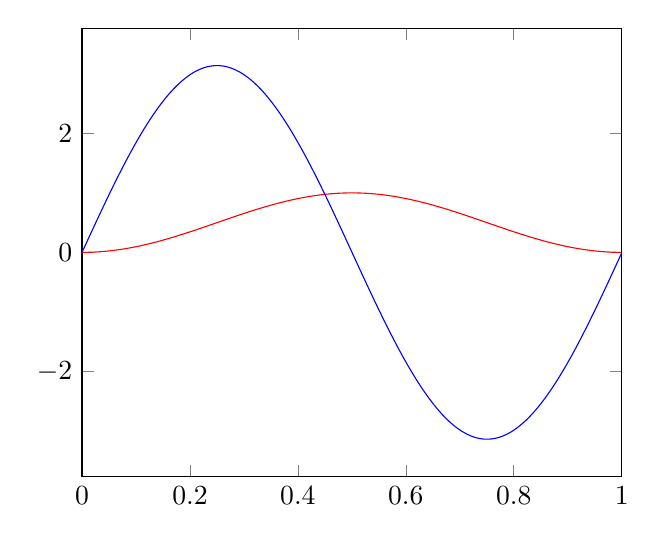
\begin{tikzpicture}
				\begin{axis}[
				clip=false,
				xmin=0,xmax=1,
				%axis lines=left,
				%axis x line=middle,
				%axis y line=left,
				]
				\addplot[domain=0:1,samples=200,red]{sin(3.14*deg(x))^2}node[right,pos=0.9]{};
				\addplot[domain=0:1,samples=200,blue]{6.28*sin(3.14*deg(x))*cos(3.14*deg(x))}node[right,pos=0.9]{};
				\end{axis}
			\end{tikzpicture}
			}
		\end{minipage}
	\end{frame}
	\begin{frame}{T-coercive elliptic problems}
	$\newline$
	\begin{definition}[T-coercivity]
		We call a sesquilinear form $\mathcal{A}(\cdot,\cdot)$ \textbf{T-coercive} on $X$ if there exists a bijective operator $T \in L(X)$ and a constant $\alpha > 0$ s.t.
		\begin{equation*}
		\mathcal{A}(Tu,u) \ge \alpha \Vert u \Vert^2_X \qquad \forall u \in X.
		\end{equation*}
	\end{definition}
	\begin{theorem}<2->[Ciarlet\footnotemark]
		If $\mathcal{A}(\cdot,\cdot)$ is T-coercive on $X$, then the corresponding variational problem is well-posed.
	\end{theorem}
	\visible<2->{
	\begin{enumerate}
		\item[\tiny 1.] \scriptsize see e.g., P. Ciarlet Jr., "T-coercivity: Application to the discretization of Helmholtz-like problems", 2012.
	\end{enumerate}
	}
	\end{frame}
	\begin{frame}{Discrete T-coercivity}
	$\newline$
	\begin{itemize}
		\item<1->[\oxarrow] T-coercivity is a \textbf{sufficient and necessary} condition for well-posedness of the weak formulation.
		\item<2->[\oxarrow] T-coercivity is \textbf{\color{red}not} automatically inherited onto the discrete level.
		\item<3->[\oxarrow] T-coercivity, at the discrete level, is a equivalent to \textbf{uniform inf-sup stability}, i.e.
		\begin{equation*}
		\inf_{v_h \in X_h} \sup_{w_h \in X_h} \frac{\vert a_h(v_h,w_h) \vert}{\Vert v_h \Vert_X \Vert w_h \Vert_X} \ge \beta > 0,
		\end{equation*}
		which guarantees the \textbf{well-posedness} of the discrete problem.
	\end{itemize}
	\end{frame}
	\begin{frame}{Compact Eigenvalue problems}
		\vspace{0.7cm}
		Considering the eigenvalue problem, find $(\lambda,P)\in \mathbb{R}\times H^1_0(\Omega)$ such that
		\begin{equation*}
			(\nabla P, \nabla Q)_{L^2} = \lambda (P,Q)_{L^2} \quad \forall Q \in H^1_0(\Omega).
		\end{equation*}
		\visible<2->{
		We can rewrite this as an eigenvalue problem associated with an operator $\mathcal{S}:H^1_0(\Omega)\to H^1_0(\Omega)$, i.e. find $(\lambda,P)\in \mathbb{R}\times H^1_0(\Omega)$ such that
		\begin{equation*}
			(\nabla \mathcal{S}f,\nabla Q) = \lambda (f,Q) \quad \forall Q \in H^1_0(\Omega).
		\end{equation*}}
		\vspace{-0.5cm}
		\visible<3->{
		\begin{block}{Elliptic regularity}
			Via elliptic regularity theory, we know that the operator $\mathcal{S}$ is compact.
			In fact, by Rellich-Kondrachov we know that $H^2(\Omega)\subset\!\subset H^1_0(\Omega)$.
		\end{block}}
	\end{frame}
	\begin{frame}{Hilbert basis}
		$\newline$
		\begin{itemize}
			\item<1->[\oxarrow] Let $(\lambda^{(i)},\Phi^{(i)})_{i\in\mathbb{N}}$ be the eigenpairs of the operator $\mathcal{S}$.
			\item<2->[\oxarrow] The eigenfunctions $(\Phi^{(i)})_{i\in\mathbb{N}}$ form a \textbf{Hilbert basis} of $H^1_0(\Omega)$.
			\item<3->[\oxarrow] We expand any $\Phi^{(i)}\in H^1_0(\Omega)$ as $P = \sum_{i\in\mathbb{N}} \Phi^{(i)}( P,\Phi^{(i)})_{H^1}$.
			\item<4->[\oxarrow] We will adopt the convection that the $\norm{\Phi^{(i)}}_{H^1}$ is unitary.
		\end{itemize}
		\visible<5->{\begin{block}{Spectral decomposition}
			$S$ is a compact operator on $H^1_0(\Omega)$, hence the eigenvalues $\lambda^{(i)}$ are \textbf{discrete} and \textbf{tend to zero}.
			Furthermore, the eigenfunctions $P^{(i)}$ form a \textbf{Hilbert basis} of $H^1_0(\Omega)$.
		\end{block}}
	\end{frame}

	\begin{frame}{T-coercivity of the Helmholtz problem}
	\vspace{1.2cm}
	\quad \oxarrow \; $\lVert \Phi^{(i)} \lVert_{H^1} = 1$ implies $\lVert \Phi^{(i)} \lVert_{L^2} = (1+\lambda^{(i)})^{-1/2}$. \\
	\vspace{-0.5cm}
	\visible<2->{
	\begin{align*}
		\mathcal{A}(P,P) &= (\nabla P,\nabla P)_{L^2} -k^2 (P,P)_{L^2(\Omega)}\\
		&= \sum_{i\in \N} P^{(i)} (\nabla \Phi^{(i)}, \nabla P)_{L^2} - k^2 P^{(i)} (\Phi^{(i)},P)_{L^2} \\
		&= \sum_{i\in \N} \lambda^{(i)} P^{(i)} (\Phi^{(i)},P)_{L^2} - k^2 P^{(i)} (\Phi^{(i)},P)_{L^2} \\
		&= \sum_{i\in \N} \lambda^{(i)} \lvert P^{(i)} \lvert^2 (\Phi^{(i)},\Phi^{(i)})_{L^2} - k^2 \lvert P^{(i)}\lvert^2 (\Phi^{(i)},\Phi^{(i)})_{L^2} \\
		&=\sum_{i \in \mathbb{N}} \left( \frac{\lambda^{(i)} - k^2}{1-\lambda^{(i)}} \right) \lvert P^{(i)}\lvert^2
	\end{align*}
	}
	\end{frame}

	\begin{frame}{T-coercivity of the Helmholtz problem}
	$\newline$
	\visible<1->{Suppose $\exists i_{\ast}$ s.t. $\lambda_1 < \dots < \lambda_{i_{\ast}} < k^2 < \lambda_{i_{\ast} + 1} < ...$}
	$\newline$
	$\newline$
	\visible<2->{
	We then construct $W := \text{span}_{0 \le i \le i_{\ast}} \{ \Phi^{(i)} \}$ and set $T := \operatorname{Id}_X - 2 P_{W}$, i.e. 
	\begin{equation*}
		T \Phi^{(i)} = \begin{cases}
		- \Phi^{(i)} & \text{if } i \le i_{\ast}, \\
		+ \Phi^{(i)} & \text{if } i > i_{\ast}.
		\end{cases}
	\end{equation*}}
	\begin{enumerate}
		\item <3->[\oxarrow] $T$ is bijective, since it is self-inverse, i.e. $T^2 = \operatorname{Id}_X$.
	\end{enumerate}
	\end{frame}
	\begin{frame}
	$\newline$
	$\newline$
	We notice that $\mathcal{A}(\cdot,\cdot)$ is T-coercive, provided $k^2$ not an eigenvalue $\lambda^{(i)}$, since
	\begin{equation*}
		\begin{aligned}
		\mathcal{A}(P,TP) &= \sum_{i \le i_{\ast}} \left( \frac{k^2 - \lambda^{(i)}}{1+\lambda^{(i)}} \right) (\Phi^{(i)})^2  + \sum_{i > i_{\ast}} \left( \frac{\lambda^{(i)} - k^2}{1+\lambda^{(i)}} \right) (\Phi^{(i)})^2  \\
		&\ge \alpha \sum_{i \in \mathbb{N}} \lambda^{(i)} (\Phi^{(i)})^2 = \alpha \Vert P \Vert^2_{H^1}, 
		\end{aligned}
	\end{equation*}
	where $\alpha = \min_{i \ge 0} \left\{ \left \vert \frac{\lambda^{(i)} - k^2}{1+\lambda^{(i)}} \right \vert \right\} > 0$.
	\end{frame}

	\begin{frame}{Weak T-coercivity}
	\vspace{0.5cm}
	\begin{definition}[weak T-coercivity]
		A linear operator $A \in L(X)$ is called \textbf{weakly T-coercive} if there exists a bijective operator $T \in L(X)$ and $K \in L(X)$ compact s.t. $T^*A + K$ is coercive. 
	\end{definition}
	\begin{itemize}
	\item<2->[\oxarrow] $A$ is T-coercive if $T^*A$ is bijective.
	\item<3->[\oxarrow] $A$ is weakly T-coercive if $T^*A + K$, $B$ bijective and $K$ compact.
	\end{itemize}
	
	\begin{lemma}<4->
	If $A$ is weakly T-coercive and injective, then $A$ is bijective. 
	\end{lemma}
	\end{frame}


	\begin{frame}{Robin boundary conditions}
	\vspace{0.8cm}
	Consider the Helmholtz problem with Robin boundary conditions, i.e. find $u \in H^1(\Omega)$ such that $\mathcal{A}(P,Q) = \prescript{}{H^{-1}}{\langle} f,Q \rangle_{H^1}$ $\forall Q \in X$, where
	\begin{equation*}
		\mathcal{A}(P,Q)\!:=\! \underbrace{(\nabla P, \nabla Q)_{L^2} \!- k (P,Q)_{L^2}}_{\mathcal{A}_0(P,Q)} {\color{gray!60!black} \!- ik \langle P, Q \rangle_{L^2(\partial \Omega)}}\! = (f , Q)_{L^2}.
	\end{equation*}
	\vspace{-0.5cm}
	\begin{block}<2->{Trace theorem}
		On bounded Lipschitz domains, the trace operator $\gamma_0 : H^1(\Omega) \to L^2(\partial \Omega)$ is compact. 
	\end{block}
	\begin{itemize}
		\item<3->[\oxarrow] The operator $\langle Ku, v \rangle_{H^1} := - i k \langle \gamma_0 u, \gamma_0 v \rangle_{L^2(\partial \Omega)}$ is compact. \\
		\item<4->[\oxarrow] $A$ is weakly T-coercive (injectivity can also be shown)
	\end{itemize}
	\end{frame}
	 
	\begin{frame}{Schatz argument}
	\vspace{0.8cm}
	We begin observing that the sesquilinear form $\mathcal{A}_0$ satisfies the \textit{G\aa rding inequality}, i.e.
	\vspace{-0.3cm }
	\begin{equation*}
		\mathcal{G}\norm{P-P_h}_{H^1_k}^2 \leq Re\left\{\mathcal{A}_0(P-P_h,P-Q_h)\right\} + k^2\norm{P-P_h}_{L^2}^2,
	\vspace{-0.5cm }
	\end{equation*}
	where we have introduced the norm $\norm{P}_{H^1_k}^2 \!:=\!\norm{\nabla P}_{L^2}^2 \!+\! k^2\norm{P}_{L^2}^2$.
	\visible<2->{
		\begin{block}{Aubin-Nitsche duality trick}
			The following bound holds,
			\begin{equation*}
				\norm{P-P_h}_{L^2} \leq M^2\psi(X_h)\norm{P-P_h}_{H^1_k},
			\end{equation*}
			where $\psi(X_h):=\underset{g\in L^2(\Omega)}{\sup}\underset{Q_h\in X_h}{\inf}\frac{\norm{g-Q_h}_{H^1_k}}{\norm{g}_{L^2}}$.
		\end{block}
	}
	\end{frame}
	\begin{frame}{Schatz argument}
		\vspace{1cm}
		Combining the G\aa rding inequality with the Aubin-Nitsche duality trick, we obtain
		\begin{equation*}
				\mathcal{G} \norm{P-P_h}_{H^1_k}^2 \leq M \norm{P-Q_h}_{H^1_k}\norm{P-P_h}_{H^1_k} + M^2k^2 \psi(X_h)^2 \norm{P-P_h}_{H^1_k}^2.
		\end{equation*}
		\visible<2->{
			Imposing the following condition on $\psi(X_h)$,
			\begin{equation}
				\psi(X_h) \leq \left(\frac{\mathcal{G}}{2k^2M^2}\right)^{\frac{1}{2}},
			\end{equation}
			we obtain the following error bound:
			\begin{equation}
				\mathcal{G}\norm{P-P_h}_{H^1_k} \leq 2M\underset{Q_h\in X_h}{\inf}\norm{P-Q_h}_{H^1_k}.
			\end{equation}
		}
	\end{frame}	
	\begin{frame}{Schatz argument}
		\vspace{1cm}
		Using \textit{Bramble-Hilbert lemma}, we can bound $\psi(X_h)$ as
		\begin{equation*}
			\psi (X_h) \leq C_\mathcal{I} h \norm{Z}_{H^2(\Omega)} \leq \left(\frac{\mathcal{G}}{2k^2M^2}\right)^{\frac{1}{2}}.
		\end{equation*}
		\vspace{-0.5cm}
		\visible<2->{
			\begin{block}{Frequency regularity estimates}
				The following regularity estimate holds $\norm{P}_{H^2}\!\leq\! (1\!+\!kC_\Omega)\norm{g}_{L^2}$, for $P\in H^2(\Omega)$ such that $-\Delta P = g$.
			\end{block}
		}
		\visible<3->{
			Combining the previous estimates we obtain,
			\vspace{-0.3cm}
			\begin{equation*}
				h \lesssim C_\mathcal{I} \left(\frac{\mathcal{G}}{2k^2M^2}\right)^{\frac{1}{2}}(1+kC_\Omega)^{-1}\sim k^{-2}.	
			\end{equation*}
		}
	\end{frame}
	\begin{frame}{Discrete T-coercivity}
	\vspace{0.4cm}
	\begin{definition}
		We call a family of sesquilinear forms $(\mathcal{A}_h)_{h>0}$ on $X_h$ \textbf{\color{red}uniformly} T$_h$-coercive, if there exists bijective operators $T_h : X_h \to X_h$ and $\alpha > 0$ independent of $h$ s.t.
		\vspace{-0.3cm}
		\begin{equation*}
		\mathcal{A}_h(P_h,T_h P_h) \ge \alpha \Vert P_h \Vert^2_{X} \qquad \forall P_h \in X_h.
		\end{equation*}
	\end{definition}
	\visible<2->{
	\oxarrow \ \normalsize If $\mathcal{A}_h$ is uniformly T$_h$-coercive, then the discrete problem is stable and quasi-optimal $\Vert P - P_h \Vert_{X} \lesssim \inf_{P_h \in X_h} \Vert P - Q_h \Vert_{X}.$}
	\\
	\visible<3->{
	\textbf{Provided} it is usually enough to show that 
	\vspace{-0.2cm}
	\begin{equation*}
		\lim_{h \to 0} \Vert T - T_h \Vert_{X} = 0,
	\end{equation*}
	but this is an asymptotic result not explicit about $h$. 
	}
	\end{frame}

	\begin{frame}{Discrete weak T-coercivity}
	\vspace{0.7cm}
	\begin{theorem}
		Let $A = B + K$, where $B$ is bijective and $K$ compact and suppose that $\operatorname{ker}(A) = \{ 0 \}$. If there exists a family of bijective operators $T_h \in \mathcal{L}(X_h)$ s.t. $B$ is \textbf{\color{red} uniformly T$_h$-coercive} on $X_h$, then there exists $h_0 > 0$ s.t. $A$ is \textbf{\color{red} uniformly T$_h$-coercive} on $X_h$ for $h < h_0$.
	\end{theorem}
	$\newline$
	\oxarrow \ \normalsize If $A$ is weakly coercive and injective, and $(T^{\ast})^{-1} B$ is uniformly T$_h$-coercive, then the discrete problem is stable and quasi-optimal
	\begin{equation*}
		\Vert P - P_h \Vert_{X} \lesssim \inf_{Q_h \in X_h} \Vert P - Q_h \Vert_{X}.
	\end{equation*}
	\end{frame}

	\begin{frame}{Discrete Helmholtz}
	\vspace{1cm}
	Find $P_h \in X_h$ such that for any $P_h\in X_h$ the following holds,
	\begin{equation*}
		\mathcal{A}(P_h,Q_h)\!:=\! \underbrace{(\nabla P_h, \nabla Q_h)_{L^2} \!- k (P_h,Q_h)_{L^2}}_{=: \mathcal{A}_0(P_h,Q_h)} {\color{gray!60!black} \!- ik \langle P_h, Q_h \rangle_{L^2(\partial \Omega)}}\! = (f , Q_h)_{L^2}.
	\end{equation*}
	\visible<2->{
	\Large \oxarrow \ \normalsize Only have to show that $\mathcal{A}_0$ is uniformly T$_h$-coercive. \\
	Define $T_h : X_h \to X_h$ through 
	\begin{equation*}
		T_h e_h^{(i)} := \begin{cases}
		- e_h^{(i)} & \text{if } i \le i_{\ast}, \\
		+ e_h^{(i)} & \text{if } i > i_{\ast}.
		\end{cases}
	\end{equation*}}
	\end{frame}
	\begin{frame}{Discrete T-coercivity of $\mathcal{A}_0$}
	\vspace{0.5cm}
	Following the same steps as before, we can expand $P_h$ in terms of the eigenfunctions of $\mathcal{S}: X_h\to X_h$, i.e. $P_h = \sum_{i \in \mathbb{N}} P_h^{(i)} \Phi_h^{(i)}$.
	\begin{equation*}
		\mathcal{A}_0(P_h,T_h P_h) := \sum_{i \le i_{\ast}} \left( \frac{k - \lambda_h^{(i)}}{1+\lambda_h^{(i)}} \right) (P_h^{(i)})^2  + \sum_{i > i_{\ast}} \left( \frac{\lambda_h^{(i)} - k}{1+\lambda_h^{(i)}} \right) (P_h^{(i)})^2.
	\end{equation*}
	\begin{itemize}
		\item<2->[\oxarrow] $\mathcal{A}_0$ is uniformly T$_h$-coercive if and only if $\lambda_h^{(i_{\ast})} < k^2$.
		\item<3->[\oxarrow] This is equivalent to ensure that $\lambda_h^{(i_{\ast})} - \lambda^{(i_{\ast})} < k^2 - \lambda^{(i_{\ast})}$ \\
	\end{itemize}
	\end{frame}

	\begin{frame}{Discrete T-coercivity of $\mathcal{A}_0$}
		\vspace{0.7cm}
		\begin{figure}
			\centering
			\only<1>{
				\includegraphics[scale=0.5]{Figures/convergence_k_10_k_12.png}
				\vspace{-0.3cm}
				\caption{
					$L^2$-error of the approximation of the Helmholtz problem with Dirichlet boundary conditions against a computed reference solution.
					$\newline$
					The vertical lines indicate when $\lambda_h^{(i_{\ast})} < k^2$.
				}
			}
			\only<2>{
				\includegraphics[scale=0.5]{Figures/convergence_k_15_k_20.png}
				\vspace{0.1cm}
				\caption{
					$L^2$-error of the approximation of the Helmholtz problem with Dirichlet boundary conditions against a computed reference solution.
					$\newline$
					The vertical lines indicate when $\lambda_h^{(i_{\ast})} < k^2$.
				}
			}
		\end{figure}
	\end{frame}

	\begin{frame}{Eigenvalue estimates}
	\vspace{1cm}
	With classical eigenvalue estimates, we get 
	\begin{equation*}
		\lambda_h^{(i_{\ast})} - \lambda^{(i_{\ast})} \le \lambda^{(i_\ast)} 4 \sqrt{i_\ast} C_{\Omega,X} C_{\mathcal{I}} h^2,
	\end{equation*}
	where the constant $C_{\Omega,X}$ and $C_{\mathcal{I}}$ are defined as follows:
	\begin{itemize}
		\item<2->[\oxarrow] $C_{\Omega,X} = C_P/\kappa$ where $C_P$ is the Poincaré constant and $\alpha$ is the coercivity constant of $-\Delta$.
		\item<3->[\oxarrow] $C_{\mathcal{I}}$ is the interpolation constant. 
	\end{itemize}
	\visible<4->{
	So to have uniform T$_h$-coercivity, we want to ensure that  
	\begin{equation*}
		h^2 < \frac{k^2 - \lambda^{(i_{\ast})}}{ 4 \sqrt{i_\ast} \lambda^{(i_\ast)} C_{\Omega,X} C_{\mathcal{I}}}.
	\end{equation*}
	}
	\end{frame}

	\begin{frame}{Quasi-optimality of $\mathcal{A}_0$}
	\vspace{0.7cm}
	\begin{minipage}{0.6\textwidth}
	\begin{theorem}
		The bilinear form $\mathcal{A}_0$ is uniformly T$_h$-coercive on $X_h$, if $h$ is chosen such that
		\vspace{-0.3cm}
		\begin{equation*}
		h^{2} < \frac{k^2 - \lambda^{(i_{\ast})}}{ 4 \sqrt{i_\ast} \lambda^{(i_\ast)} C_{\Omega,X} C_{\mathcal{I}}}.
		\end{equation*}
	\end{theorem}
	\end{minipage}
	\,
	\begin{minipage}{0.3\textwidth}
	\begin{figure}
		\visible<2->{
		\centering
		\vspace{1.cm}
		\includegraphics[scale=0.4]{Figures/eigenvalue_estimates.png}
		}
	\end{figure}
	\end{minipage}
	\vspace{0.5cm}
	\begin{itemize}
		\item<3->[\oxarrow] This guarantees that the discrete problem is quasi-optimal provided $h$ is small enough.
	\end{itemize}
	\end{frame}

	\begin{frame}{Adaptive scheme}
	\vspace{1cm}
	Construct the mesh, with the minimal number of elements, that guarantees the quasi-optimality of the Helmholtz problem:
	\begin{enumerate}
		\item<2->[\oxarrow] \textbf{Determine $i_{\ast}$:} either we know the eigenvalues, or we have to approximate them well enough (but we can choose any method we like to do this). 
		\item<3->[\oxarrow] \textbf{Solving the Laplace eigenvalue problem adaptively:} Solve the Laplace eigenvalue problem on a sequence of refined meshes and check whether $k^2 - \lambda_h^{(i_{\ast})} < 0$. If yes, we can stop because $h$ is small enough s.t. we have uniform T$_h$-coercivity. (needs to use the same discretization as for Helmholtz)
		\item<4->[\oxarrow] \textbf{Solve the Helmholtz problem.}
	\end{enumerate}
	\end{frame}
	\begin{frame}{Adpative scheme: numerical examples}
		\vspace{0.7cm}
		\only<1>{
		\begin{figure}
			\centering
			\includegraphics[scale=0.6]{Figures/pitch_uniform_step_1.png}
		\end{figure}
		}
		\only<2>{
		\begin{figure}
			\centering
			\includegraphics[scale=0.6]{Figures/pitch_uniform_step_2.png}
		\end{figure}
		}
		\only<3>{
		\begin{figure}
			\centering
			\includegraphics[scale=0.6]{Figures/pitch_uniform_step_3.png}
		\end{figure}
		}
		\only<4>{
		\begin{figure}
			\centering
			\includegraphics[scale=0.6]{Figures/pitch_uniform_step_4.png}
		\end{figure}
		}
	\end{frame}
	\begin{frame}{Adaptive$^2$ scheme}
	\begin{itemize}
		\item[\oxarrow] In the adaptive scheme, we use a \textbf{Babuška--Rheinboldt} estimator to adaptively refine the mesh.
		\item[\oxarrow] The main idea is to use the \textbf{Babuška--Rheinboldt} estimator not one the desired solution or on a specific eigenfunction, but rather on the first $i_{\ast}+\ell$ eigenfunctions, i.e.
		\begin{equation*}
			\eta_K\! =\! i_{\ast}^{-1}\!\!\sum_{i = 1}^{i_{\ast}+\ell}\! h^2_K \Vert \Delta e_h^{(i)} \!+\!\lambda_h^{(i)} e_h^{(i)} \Vert^2_{L^2(K)} \!+\! \frac{h_K}{2} \Vert \nabla e_h^{(i)}\! \cdot n \Vert^2_{L^2(\partial K \setminus \partial \Omega)}.
		\end{equation*}
		\item[\oxarrow] We then refine the mesh in the elements where the indicator is larger. We can also adapt a \textbf{D\"orfler marking} strategy.
	\end{itemize} 
	\end{frame}
	\begin{frame}{Adpative$^2$ scheme: numerical examples}
		\vspace{0.7cm}
		\only<1>{
		\begin{figure}
			\centering
			\includegraphics[scale=0.6]{Figures/pitch_adpt_step_1.png}
		\end{figure}
		}
		\only<2>{
		\begin{figure}
			\centering
			\includegraphics[scale=0.6]{Figures/pitch_adpt_step_2.png}
		\end{figure}
		}
		\only<3>{
		\begin{figure}
			\centering
			\includegraphics[scale=0.6]{Figures/pitch_adpt_step_3.png}
		\end{figure}
		}
		\only<4>{
		\begin{figure}
			\centering
			\includegraphics[scale=0.6]{Figures/pitch_adpt_step_4.png}
		\end{figure}
		}
	\end{frame}
\end{document}


\pgfdeclareimage[width=\paperwidth]{titlebackground}{Images/title-slide-background.png}
\setbeamerfont{subtitle}{size=\tiny}
\setbeamertemplate{endpage}{
	\begin{picture}(0,0)
		\scalebox{1.01}{
		\put(-28.5,-163){%
			\pgfuseimage{titlebackground}
		}
		}
		\put(0,-115){%
			\begin{minipage}[b][4.5cm][t]{0.5\textwidth}
				\color{white}
				\usebeamerfont{title}
				{\textbf{Thank Your} \\ \textbf{For You Attention !}}
			\end{minipage}
		}
	\end{picture}
}
\setbeamertemplate{title page}{
	\begin{picture}(0,0)
		\scalebox{1.01}{
			\put(-28.5,-163){%
				\pgfuseimage{titlebackground}
			}
		}
		\put(0,-60){%
			\begin{minipage}[b][4.5cm][t]{0.7\textwidth}
				\color{white}
				\usebeamerfont{title}
				{\inserttitle\\[0.9cm]}
				\usebeamerfont{subtitle}
				{\insertauthor\par}
				{\insertinstitute\\[0.3cm]}
				{\insertdate}
			\end{minipage}
		}
	\end{picture}
}


%% General slide formatting %%

\definecolor{oxfordblue}{RGB}{4,30,66}
\definecolor{oxfordred}{RGB}{207,48,42}

\pgfdeclareimage[width=0.9cm]{oxfordlogo}{Images/oxford-logo.png}
\pgfdeclareimage[width=1cm]{mathslogo}{Images/mathematics-logo.png}
\pgfdeclareimage[width=1.2cm]{ngslogo}{Images/ngs-logo.png}
\pgfdeclareimage[width=1.2cm]{petsclogo}{Images/petsc-logo.png}
\pgfdeclareimage[width=1.2cm]{firedrakelogo}{Images/firedrake-logo.png}

\setbeamertemplate{headline}
{%
	\begin{picture}(0,0)
		\put(314,-50){%
			\pgfuseimage{oxfordlogo}
		}
		\put(20,-55){%
			\rule{320pt}{0.4pt}
		}
	\end{picture}
}
\def\ngshead{
	\begin{picture}(0,0)
		\put(278,0){%
			\pgfuseimage{ngslogo}
		}
		\put(-8,-5){%
			\rule{325pt}{0.4pt}
		}
	\end{picture}
}
\def\petschead{
	\begin{picture}(0,0)
		\put(278,0){%
			\pgfuseimage{petsclogo}
		}
		\put(-8,-5){%
			\rule{325pt}{0.4pt}
		}
	\end{picture}
}
\def\firedrakehead{
	\begin{picture}(0,0)
		\put(278,0){%
			\pgfuseimage{firedrakelogo}
		}
		\put(-8,-5){%
			\rule{325pt}{0.4pt}
		}
	\end{picture}
}
\setbeamertemplate{frametitle}
{%
	\begin{picture}(0,0)
		\put(-8,-20){%
			\normalsize\textbf{\color{oxfordblue}\insertframetitle}
		}
		\put(-8,-32){%
			\normalsize\textbf{\color{oxfordblue}\insertframesubtitle}
		}
	\end{picture}
}

\setbeamertemplate{footline}
{%
	\begin{picture}(0,0)
		\put(20,30){%
			\rule{320pt}{0.4pt}
		}
		\put(20,14){%
			\pgfuseimage{mathslogo}
		}
		\put(100,14){%
			\color{oxfordblue}\insertshortdate
		}
		\put(160,14){%
			\color{oxfordblue}\insertshorttitle
		}
		\put(337,14){%
			\color{oxfordblue}\insertframenumber
		}
	\end{picture}%
}
\def\footer{
	\begin{picture}(0,0)
		\put(-308,-75){%
			\rule{325pt}{0.4pt}
		}
		\put(-308,-91){%
			\pgfuseimage{mathslogo}
		}
		\put(-228,-91){%
			\color{oxfordblue}\tiny\insertshortdate
		}
		\put(-168,-91){%
			\color{oxfordblue}\tiny\insertshorttitle
		}
		\put(9,-91){%
			\color{oxfordblue}\tiny\insertframenumber
		}
	\end{picture}
}

\setbeamercolor{block title}{bg=oxfordblue!30,fg=black}
\setbeamercolor{palette primary}{bg=oxfordblue,fg=white}

\definecolor{codegreen}{rgb}{0,0.6,0}
\definecolor{codegray}{rgb}{0.5,0.5,0.5}
\definecolor{codepurple}{rgb}{0.58,0,0.82}
\definecolor{backcolour}{rgb}{0.95,0.95,0.92}

\lstdefinestyle{mystyle}{
	%backgroundcolor=\color{backcolour},   
	commentstyle=\color{codegray},
	keywordstyle=\color{oxfordblue},
	numberstyle=\tiny\color{codegray},
	stringstyle=\color{codegreen},
	basicstyle=\ttfamily\footnotesize,
	breakatwhitespace=false,         
	breaklines=true,                 
	captionpos=b,                    
	keepspaces=true,                 
	numbers=left,                    
	numbersep=5pt,                  
	showspaces=false,                
	showstringspaces=false,
	showtabs=false,                  
	tabsize=2
}
\AtBeginSection[]{
  \begin{frame}
  \vfill
  \centering
  \begin{beamercolorbox}[sep=8pt,center,shadow=true,rounded=true]{title}
    \usebeamerfont{title}\insertsectionhead\par%
  \end{beamercolorbox}
  \vfill
  \end{frame}
}

\lstset{style=mystyle}

%Specific macros
\newcommand{\oxarrow}{\color{oxfordblue}$\blacktriangleright$}
\newcommand{\N}{\mathbb{N}}

%% Information (author, title, etc.) %%
\title[Helmholtz]{Quasi-optimality of FEMs for the Helmholtz equation}
\author%
{%
	\sc{T.~van~Beeck$^\dag$}, \underline{\sc{U.~Zerbinati}}$^*$\\
}
\institute%
{%
	* \textit{Mathematical Institute}\\
	\;\textit{University of Oxford}\\
	$\newline$
	$\dag$ \textit{Institute for Numerical and Applied Mathematics}\\
	\;\textit{University of G\"ottingen}\\	
}

\date[\textbf{PYSANUM}]{} 



%% Content of slides %%

\begin{document}
	\begin{frame}[plain]
		\titlepage
	\end{frame}

	\begin{frame}{The wave equation}
		\visible<1->{The \textbf{wave equation} is a second-order linear partial differential equation for the description of waves.}
		$\newline$
		$\newline$
		\visible<2->{In particular, it describes the evolution of an \textbf{excess pressure} $p_\delta$ in a medium with speed of sound $c$.}
		\visible<3->{
		\begin{equation}
			\begin{aligned}
				\partial_t^2 p_\delta - c^2\Delta p_\delta &= f \quad &\text{in } \;\;\;\Omega \times (0,T), \\
				p_\delta &= 0 \quad &\text{on } \partial \Omega \times (0,T), \\
				p_\delta(\cdot,0) &= p_0(\cdot), \quad & \partial_t p_\delta(\cdot,0) = \dot{p}_0(\cdot).
			\end{aligned}
		\end{equation}}
	\end{frame}

	\begin{frame}{Time harmonic solutions of the wave equation}
		$\newline$
		\visible<1->{The \textbf{time harmonic solutions} of the wave equation are of the form}
		\begin{equation}
			p^{(\delta)}(\cdot,t) = \Re\left\{ P(\cdot) e^{-i\omega t} \right\},
		\end{equation}
		\visible<1->{where $P:\Omega\to \mathbb{C}$ and $\omega$ is the \textbf{angular frequency}.}
		$\newline$
		\visible<2->{Substituting this ansatz into the wave equation, we obtain the \textbf{Helmholtz equation}
		\begin{equation}
			\begin{aligned}
				- \Delta P - k^2 P &= F \quad &\text{in } \;\;\;\Omega, \\
				u &= 0 \quad &\text{on } \partial \Omega,
			\end{aligned}
		\end{equation}}
		\visible<2->{where $k = \omega/c$ is the \textbf{wave number} and $F = \Re\left\{f(\cdot,t)e^{-i\omega t}\right\}$.}
	\end{frame}
	\begin{frame}{The weak formulation}
		$\newline$
		\visible<1->{The \textbf{weak formulation} of the Helmholtz equation is to find $u \in H^1_0(\Omega)$ such that
		\begin{equation}
			\begin{aligned}
				(\nabla P, \nabla Q)_{L^2} - k^2 (P,Q)_{L^2} &= \prescript{}{H^{-1}}{\langle} F,Q \rangle_{H^1_0} \quad \forall Q \in H^1_0(\Omega),
			\end{aligned}
		\end{equation}
		where $(\cdot,\cdot)_{L^2}$ denotes the $L^2$ inner product.}
		$\newline$
		$\newline$
		\visible<2->{The weak formulation of the Helmholtz equation is \textbf{elliptic}, hence we can make use of \textbf{elliptic regularity theory}.}
		$\newline$
		$\newline$
		\visible<3->{The Helmholtz problem is \textbf{ill-posed} if $k^2$ is an eigenvalue of the Laplacian, in the sense that the solution $P$ is not uniquely determined by the data $F$.}
	\end{frame}
	\begin{frame}{Finite element discretization}
		\vspace{0.8cm}
		\visible<1->{The \textbf{finite element discretization} of the Helmholtz equation is to find $u_h \in X_h$ such that
		\begin{equation}
			\begin{aligned}
				(\nabla P_h, \nabla Q_h)_{L^2} - k^2 (P_h,Q_h)_{L^2} &= (F,Q_h)_{L^2} \quad \forall Q_h \in X_h,
			\end{aligned}
		\end{equation}
		where $X_h \subset H^1_0(\Omega)$ is a finite-dimensional subspace.}
		\begin{itemize}
			\item<2->[\oxarrow] We discretize the domain $\Omega$ into a mesh of elements $\{\mathcal{T}_h\}_{h>0}$.
			\item<3->[\oxarrow] We choose as $X_h$ the space of piecewise linear polynomial functions on the mesh, i.e.
			\begin{equation*}
				X_h := \{ v \in L^2(\Omega) : v \vert_{\tau} \in \mathcal{P}^1(\tau) \ \forall \tau \in T_h \} \cap H^1_0(\Omega) \subset H^1_0(\Omega).
			\end{equation*}
			\item<4->[\oxarrow] We obtain a \textbf{linear system} of the form $\underline{\underline{\mathcal{A}}} \,\underline{P}_h = \underline{F}$.
		\end{itemize}	
	\end{frame}
	\begin{frame}{A motivating example}
		$\newline$
		$\newline$
		\begin{equation}
			P(\cdot) = \sin(\pi \omega \cdot), \qquad \omega = 16
		\end{equation}
		$\newline$
		\only<2>{
			\begin{minipage}{0.3\textwidth}
				\begin{figure}
					\centering
					\includegraphics[scale=0.3]{Figures/proj_N_6_omega_16.png}
					\caption{$L^2$ projection}
				\end{figure}
			\end{minipage}
			\begin{minipage}{0.3\textwidth}
				\begin{figure}
					\centering
					\includegraphics[scale=0.3]{Figures/poisson_N_6_omega_16.png}
					\caption{$k=0$}
				\end{figure}
			\end{minipage}
			\begin{minipage}{0.3\textwidth}
				\begin{figure}
					\centering
					\includegraphics[scale=0.3]{Figures/helmholtz_N_6_omega_16.png}
					\caption{$k=256$}
				\end{figure}
			\end{minipage}
		}
		\only<3>{
			\begin{minipage}{0.3\textwidth}
				\begin{figure}
					\centering
					\includegraphics[scale=0.3]{Figures/proj_N_24_omega_16.png}
					\caption{$L^2$ projection}
				\end{figure}
			\end{minipage}
			\begin{minipage}{0.3\textwidth}
				\begin{figure}
					\centering
					\includegraphics[scale=0.3]{Figures/poisson_N_24_omega_16.png}
					\caption{$k=0$}
				\end{figure}
			\end{minipage}
			\begin{minipage}{0.3\textwidth}
				\begin{figure}
					\centering
					\includegraphics[scale=0.3]{Figures/helmholtz_N_24_omega_16.png}
					\caption{$k=256$}
				\end{figure}
			\end{minipage}
		}
		\only<4>{
			\begin{minipage}{0.3\textwidth}
				\begin{figure}
					\centering
					\includegraphics[scale=0.3]{Figures/proj_N_48_omega_16.png}
					\caption{$L^2$ projection}
				\end{figure}
			\end{minipage}
			\begin{minipage}{0.3\textwidth}
				\begin{figure}
					\centering
					\includegraphics[scale=0.3]{Figures/poisson_N_48_omega_16.png}
					\caption{$k=0$}
				\end{figure}
			\end{minipage}
			\begin{minipage}{0.3\textwidth}
				\begin{figure}
					\centering
					\includegraphics[scale=0.3]{Figures/helmholtz_N_48_omega_16.png}
					\caption{$k=256$}
				\end{figure}
			\end{minipage}
		}
	\end{frame}

	\begin{frame}{Coercive elliptic problems}
	\vspace{0.8cm}
	\begin{definition}<1->[Coercivity]
		We call a sesquilinear form $\mathcal{A}:X\times X\to \mathbb{C}$ \textbf{coercive} on $X$ if there exists a constant $\alpha > 0$ such that
		\begin{equation*}
		\mathcal{A}(P,P) \ge \alpha \Vert P \Vert^2_X \qquad \forall P \in X. 
		\end{equation*}
	\end{definition}
	\begin{theorem}<2->[Lax-Milgram]
		If $\mathcal{A}:X\times X\to\mathbb{C}$ is coercive on $X$, then the variational problem 
		\begin{equation*}
		\text{find } P \in X \text{ such that } \mathcal{A}(P,Q) = \prescript{}{X'}{\langle} f,Q\rangle_{X} \quad \forall Q \in X
		\end{equation*}
		is \textbf{well-posed} for all $f \in X'$.
	\end{theorem}
	\end{frame}
	\begin{frame}{Discrete coercive problems}
		$\newline$
		\begin{itemize}
			\item [\oxarrow] Via Lax-Milgram, we also know that the discrete problem is well-posed if the bilinear form is coercive.
		\end{itemize}
		\begin{block}<2->{Cea's lemma}
			Let $\mathcal{A}:X \times X\to\mathbb{C}$ be coercive on $X$ and let $P\in X$ be the solution of the continuous variational problem. Then the solution $P_h\in X_h$ of the discrete variational problem satisfies
			\begin{equation*}
			\Vert P-P_h \Vert_X \le \frac{M}{\alpha} \inf_{Q_h \in X_h} \Vert P - Q_h \Vert_X,
			\end{equation*}
			where $M$ is the continuity constant of $\mathcal{A}$. 

		\end{block}
	\end{frame}
	\begin{frame}{Lack of coercivity of the Helmholtz problem}
		$\newline$
		Consider the function $P(x) = \sin(\pi \omega x)$.
		\begin{minipage}{0.6\textwidth}
		\begin{align}
		&\norm{P}^2_{L^2\left([0,1]\right)}\! =\! \int_0^1 \sin^2(\pi \omega x) = \frac{1}{2}\\
		&\norm{P'}^2_{L^2\left([0,1]\right)}\! =\! \int_0^1 2\pi\sin(\pi \omega x)\cos(\pi\omega x)
		\end{align}
		notice that the last integral vanishes for $\omega \in \mathbb{N}$, on the interval $[0,1]$.
		\end{minipage}
		\begin{minipage}{0.35\textwidth}
			\scalebox{0.5}[0.5]{
			  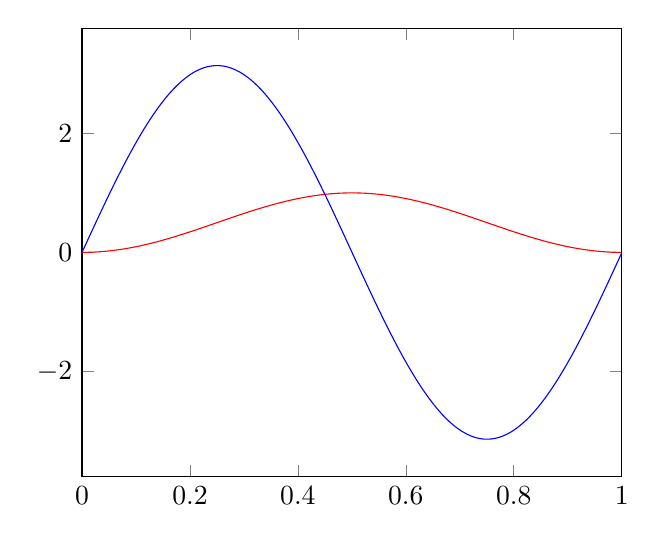
\begin{tikzpicture}
				\begin{axis}[
				clip=false,
				xmin=0,xmax=1,
				%axis lines=left,
				%axis x line=middle,
				%axis y line=left,
				]
				\addplot[domain=0:1,samples=200,red]{sin(3.14*deg(x))^2}node[right,pos=0.9]{};
				\addplot[domain=0:1,samples=200,blue]{6.28*sin(3.14*deg(x))*cos(3.14*deg(x))}node[right,pos=0.9]{};
				\end{axis}
			\end{tikzpicture}
			}
		\end{minipage}
	\end{frame}
	\begin{frame}{T-coercive elliptic problems}
	$\newline$
	\begin{definition}[T-coercivity]
		We call a sesquilinear form $\mathcal{A}(\cdot,\cdot)$ \textbf{T-coercive} on $X$ if there exists a bijective operator $T \in L(X)$ and a constant $\alpha > 0$ s.t.
		\begin{equation*}
		\mathcal{A}(Tu,u) \ge \alpha \Vert u \Vert^2_X \qquad \forall u \in X.
		\end{equation*}
	\end{definition}
	\begin{theorem}<2->[Ciarlet\footnotemark]
		If $\mathcal{A}(\cdot,\cdot)$ is T-coercive on $X$, then the corresponding variational problem is well-posed.
	\end{theorem}
	\visible<2->{
	\begin{enumerate}
		\item[\tiny 1.] \scriptsize see e.g., P. Ciarlet Jr., "T-coercivity: Application to the discretization of Helmholtz-like problems", 2012.
	\end{enumerate}
	}
	\end{frame}
	\begin{frame}{Discrete T-coercivity}
	$\newline$
	\begin{itemize}
		\item<1->[\oxarrow] T-coercivity is a \textbf{sufficient and necessary} condition for well-posedness of the weak formulation.
		\item<2->[\oxarrow] T-coercivity is \textbf{\color{red}not} automatically inherited onto the discrete level.
		\item<3->[\oxarrow] T-coercivity, at the discrete level, is a equivalent to \textbf{uniform inf-sup stability}, i.e.
		\begin{equation*}
		\inf_{v_h \in X_h} \sup_{w_h \in X_h} \frac{\vert a_h(v_h,w_h) \vert}{\Vert v_h \Vert_X \Vert w_h \Vert_X} \ge \beta > 0,
		\end{equation*}
		which guarantees the \textbf{well-posedness} of the discrete problem.
	\end{itemize}
	\end{frame}
	\begin{frame}{Compact Eigenvalue problems}
		\vspace{0.7cm}
		Considering the eigenvalue problem, find $(\lambda,P)\in \mathbb{R}\times H^1_0(\Omega)$ such that
		\begin{equation*}
			(\nabla P, \nabla Q)_{L^2} = \lambda (P,Q)_{L^2} \quad \forall Q \in H^1_0(\Omega).
		\end{equation*}
		\visible<2->{
		We can rewrite this as an eigenvalue problem associated with an operator $\mathcal{S}:H^1_0(\Omega)\to H^1_0(\Omega)$, i.e. find $(\lambda,P)\in \mathbb{R}\times H^1_0(\Omega)$ such that
		\begin{equation*}
			(\nabla \mathcal{S}f,\nabla Q) = \lambda (f,Q) \quad \forall Q \in H^1_0(\Omega).
		\end{equation*}}
		\vspace{-0.5cm}
		\visible<3->{
		\begin{block}{Elliptic regularity}
			Via elliptic regularity theory, we know that the operator $\mathcal{S}$ is compact.
			In fact, by Rellich-Kondrachov we know that $H^2(\Omega)\subset\!\subset H^1_0(\Omega)$.
		\end{block}}
	\end{frame}
	\begin{frame}{Hilbert basis}
		$\newline$
		\begin{itemize}
			\item<1->[\oxarrow] Let $(\lambda^{(i)},\Phi^{(i)})_{i\in\mathbb{N}}$ be the eigenpairs of the operator $\mathcal{S}$.
			\item<2->[\oxarrow] The eigenfunctions $(\Phi^{(i)})_{i\in\mathbb{N}}$ form a \textbf{Hilbert basis} of $H^1_0(\Omega)$.
			\item<3->[\oxarrow] We expand any $\Phi^{(i)}\in H^1_0(\Omega)$ as $P = \sum_{i\in\mathbb{N}} \Phi^{(i)}( P,\Phi^{(i)})_{H^1}$.
			\item<4->[\oxarrow] We will adopt the convection that the $\norm{\Phi^{(i)}}_{H^1}$ is unitary.
		\end{itemize}
		\visible<5->{\begin{block}{Spectral decomposition}
			$S$ is a compact operator on $H^1_0(\Omega)$, hence the eigenvalues $\lambda^{(i)}$ are \textbf{discrete} and \textbf{tend to zero}.
			Furthermore, the eigenfunctions $P^{(i)}$ form a \textbf{Hilbert basis} of $H^1_0(\Omega)$.
		\end{block}}
	\end{frame}

	\begin{frame}{T-coercivity of the Helmholtz problem}
	\vspace{1.2cm}
	\quad \oxarrow \; $\lVert \Phi^{(i)} \lVert_{H^1} = 1$ implies $\lVert \Phi^{(i)} \lVert_{L^2} = (1+\lambda^{(i)})^{-1/2}$. \\
	\vspace{-0.5cm}
	\visible<2->{
	\begin{align*}
		\mathcal{A}(P,P) &= (\nabla P,\nabla P)_{L^2} -k^2 (P,P)_{L^2(\Omega)}\\
		&= \sum_{i\in \N} P^{(i)} (\nabla \Phi^{(i)}, \nabla P)_{L^2} - k^2 P^{(i)} (\Phi^{(i)},P)_{L^2} \\
		&= \sum_{i\in \N} \lambda^{(i)} P^{(i)} (\Phi^{(i)},P)_{L^2} - k^2 P^{(i)} (\Phi^{(i)},P)_{L^2} \\
		&= \sum_{i\in \N} \lambda^{(i)} \lvert P^{(i)} \lvert^2 (\Phi^{(i)},\Phi^{(i)})_{L^2} - k^2 \lvert P^{(i)}\lvert^2 (\Phi^{(i)},\Phi^{(i)})_{L^2} \\
		&=\sum_{i \in \mathbb{N}} \left( \frac{\lambda^{(i)} - k^2}{1-\lambda^{(i)}} \right) \lvert P^{(i)}\lvert^2
	\end{align*}
	}
	\end{frame}

	\begin{frame}{T-coercivity of the Helmholtz problem}
	$\newline$
	\visible<1->{Suppose $\exists i_{\ast}$ s.t. $\lambda_1 < \dots < \lambda_{i_{\ast}} < k^2 < \lambda_{i_{\ast} + 1} < ...$}
	$\newline$
	$\newline$
	\visible<2->{
	We then construct $W := \text{span}_{0 \le i \le i_{\ast}} \{ \Phi^{(i)} \}$ and set $T := \operatorname{Id}_X - 2 P_{W}$, i.e. 
	\begin{equation*}
		T \Phi^{(i)} = \begin{cases}
		- \Phi^{(i)} & \text{if } i \le i_{\ast}, \\
		+ \Phi^{(i)} & \text{if } i > i_{\ast}.
		\end{cases}
	\end{equation*}}
	\begin{enumerate}
		\item <3->[\oxarrow] $T$ is bijective, since it is self-inverse, i.e. $T^2 = \operatorname{Id}_X$.
	\end{enumerate}
	\end{frame}
	\begin{frame}
	$\newline$
	$\newline$
	We notice that $\mathcal{A}(\cdot,\cdot)$ is T-coercive, provided $k^2$ not an eigenvalue $\lambda^{(i)}$, since
	\begin{equation*}
		\begin{aligned}
		\mathcal{A}(P,TP) &= \sum_{i \le i_{\ast}} \left( \frac{k^2 - \lambda^{(i)}}{1+\lambda^{(i)}} \right) (\Phi^{(i)})^2  + \sum_{i > i_{\ast}} \left( \frac{\lambda^{(i)} - k^2}{1+\lambda^{(i)}} \right) (\Phi^{(i)})^2  \\
		&\ge \alpha \sum_{i \in \mathbb{N}} \lambda^{(i)} (\Phi^{(i)})^2 = \alpha \Vert P \Vert^2_{H^1}, 
		\end{aligned}
	\end{equation*}
	where $\alpha = \min_{i \ge 0} \left\{ \left \vert \frac{\lambda^{(i)} - k^2}{1+\lambda^{(i)}} \right \vert \right\} > 0$.
	\end{frame}

	\begin{frame}{Weak T-coercivity}
	\vspace{0.5cm}
	\begin{definition}[weak T-coercivity]
		A linear operator $A \in L(X)$ is called \textbf{weakly T-coercive} if there exists a bijective operator $T \in L(X)$ and $K \in L(X)$ compact s.t. $T^*A + K$ is coercive. 
	\end{definition}
	\begin{itemize}
	\item<2->[\oxarrow] $A$ is T-coercive if $T^*A$ is bijective.
	\item<3->[\oxarrow] $A$ is weakly T-coercive if $T^*A + K$, $B$ bijective and $K$ compact.
	\end{itemize}
	
	\begin{lemma}<4->
	If $A$ is weakly T-coercive and injective, then $A$ is bijective. 
	\end{lemma}
	\end{frame}


	\begin{frame}{Robin boundary conditions}
	\vspace{0.8cm}
	Consider the Helmholtz problem with Robin boundary conditions, i.e. find $u \in H^1(\Omega)$ such that $\mathcal{A}(P,Q) = \prescript{}{H^{-1}}{\langle} f,Q \rangle_{H^1}$ $\forall Q \in X$, where
	\begin{equation*}
		\mathcal{A}(P,Q)\!:=\! \underbrace{(\nabla P, \nabla Q)_{L^2} \!- k (P,Q)_{L^2}}_{\mathcal{A}_0(P,Q)} {\color{gray!60!black} \!- ik \langle P, Q \rangle_{L^2(\partial \Omega)}}\! = (f , Q)_{L^2}.
	\end{equation*}
	\vspace{-0.5cm}
	\begin{block}<2->{Trace theorem}
		On bounded Lipschitz domains, the trace operator $\gamma_0 : H^1(\Omega) \to L^2(\partial \Omega)$ is compact. 
	\end{block}
	\begin{itemize}
		\item<3->[\oxarrow] The operator $\langle Ku, v \rangle_{H^1} := - i k \langle \gamma_0 u, \gamma_0 v \rangle_{L^2(\partial \Omega)}$ is compact. \\
		\item<4->[\oxarrow] $A$ is weakly T-coercive (injectivity can also be shown)
	\end{itemize}
	\end{frame}
	 
	\begin{frame}{Schatz argument}
	\vspace{0.8cm}
	We begin observing that the sesquilinear form $\mathcal{A}_0$ satisfies the \textit{G\aa rding inequality}, i.e.
	\vspace{-0.3cm }
	\begin{equation*}
		\mathcal{G}\norm{P-P_h}_{H^1_k}^2 \leq Re\left\{\mathcal{A}_0(P-P_h,P-Q_h)\right\} + k^2\norm{P-P_h}_{L^2}^2,
	\vspace{-0.5cm }
	\end{equation*}
	where we have introduced the norm $\norm{P}_{H^1_k}^2 \!:=\!\norm{\nabla P}_{L^2}^2 \!+\! k^2\norm{P}_{L^2}^2$.
	\visible<2->{
		\begin{block}{Aubin-Nitsche duality trick}
			The following bound holds,
			\begin{equation*}
				\norm{P-P_h}_{L^2} \leq M^2\psi(X_h)\norm{P-P_h}_{H^1_k},
			\end{equation*}
			where $\psi(X_h):=\underset{g\in L^2(\Omega)}{\sup}\underset{Q_h\in X_h}{\inf}\frac{\norm{g-Q_h}_{H^1_k}}{\norm{g}_{L^2}}$.
		\end{block}
	}
	\end{frame}
	\begin{frame}{Schatz argument}
		\vspace{1cm}
		Combining the G\aa rding inequality with the Aubin-Nitsche duality trick, we obtain
		\begin{equation*}
				\mathcal{G} \norm{P-P_h}_{H^1_k}^2 \leq M \norm{P-Q_h}_{H^1_k}\norm{P-P_h}_{H^1_k} + M^2k^2 \psi(X_h)^2 \norm{P-P_h}_{H^1_k}^2.
		\end{equation*}
		\visible<2->{
			Imposing the following condition on $\psi(X_h)$,
			\begin{equation}
				\psi(X_h) \leq \left(\frac{\mathcal{G}}{2k^2M^2}\right)^{\frac{1}{2}},
			\end{equation}
			we obtain the following error bound:
			\begin{equation}
				\mathcal{G}\norm{P-P_h}_{H^1_k} \leq 2M\underset{Q_h\in X_h}{\inf}\norm{P-Q_h}_{H^1_k}.
			\end{equation}
		}
	\end{frame}	
	\begin{frame}{Schatz argument}
		\vspace{1cm}
		Using \textit{Bramble-Hilbert lemma}, we can bound $\psi(X_h)$ as
		\begin{equation*}
			\psi (X_h) \leq C_\mathcal{I} h \norm{Z}_{H^2(\Omega)} \leq \left(\frac{\mathcal{G}}{2k^2M^2}\right)^{\frac{1}{2}}.
		\end{equation*}
		\vspace{-0.5cm}
		\visible<2->{
			\begin{block}{Frequency regularity estimates}
				The following regularity estimate holds $\norm{P}_{H^2}\!\leq\! (1\!+\!kC_\Omega)\norm{g}_{L^2}$, for $P\in H^2(\Omega)$ such that $-\Delta P = g$.
			\end{block}
		}
		\visible<3->{
			Combining the previous estimates we obtain,
			\vspace{-0.3cm}
			\begin{equation*}
				h \lesssim C_\mathcal{I} \left(\frac{\mathcal{G}}{2k^2M^2}\right)^{\frac{1}{2}}(1+kC_\Omega)^{-1}\sim k^{-2}.	
			\end{equation*}
		}
	\end{frame}
	\begin{frame}{Discrete T-coercivity}
	\vspace{0.4cm}
	\begin{definition}
		We call a family of sesquilinear forms $(\mathcal{A}_h)_{h>0}$ on $X_h$ \textbf{\color{red}uniformly} T$_h$-coercive, if there exists bijective operators $T_h : X_h \to X_h$ and $\alpha > 0$ independent of $h$ s.t.
		\vspace{-0.3cm}
		\begin{equation*}
		\mathcal{A}_h(P_h,T_h P_h) \ge \alpha \Vert P_h \Vert^2_{X} \qquad \forall P_h \in X_h.
		\end{equation*}
	\end{definition}
	\visible<2->{
	\oxarrow \ \normalsize If $\mathcal{A}_h$ is uniformly T$_h$-coercive, then the discrete problem is stable and quasi-optimal $\Vert P - P_h \Vert_{X} \lesssim \inf_{P_h \in X_h} \Vert P - Q_h \Vert_{X}.$}
	\\
	\visible<3->{
	\textbf{Provided} it is usually enough to show that 
	\vspace{-0.2cm}
	\begin{equation*}
		\lim_{h \to 0} \Vert T - T_h \Vert_{X} = 0,
	\end{equation*}
	but this is an asymptotic result not explicit about $h$. 
	}
	\end{frame}

	\begin{frame}{Discrete weak T-coercivity}
	\vspace{0.7cm}
	\begin{theorem}
		Let $A = B + K$, where $B$ is bijective and $K$ compact and suppose that $\operatorname{ker}(A) = \{ 0 \}$. If there exists a family of bijective operators $T_h \in \mathcal{L}(X_h)$ s.t. $B$ is \textbf{\color{red} uniformly T$_h$-coercive} on $X_h$, then there exists $h_0 > 0$ s.t. $A$ is \textbf{\color{red} uniformly T$_h$-coercive} on $X_h$ for $h < h_0$.
	\end{theorem}
	$\newline$
	\oxarrow \ \normalsize If $A$ is weakly coercive and injective, and $(T^{\ast})^{-1} B$ is uniformly T$_h$-coercive, then the discrete problem is stable and quasi-optimal
	\begin{equation*}
		\Vert P - P_h \Vert_{X} \lesssim \inf_{Q_h \in X_h} \Vert P - Q_h \Vert_{X}.
	\end{equation*}
	\end{frame}

	\begin{frame}{Discrete Helmholtz}
	\vspace{1cm}
	Find $P_h \in X_h$ such that for any $P_h\in X_h$ the following holds,
	\begin{equation*}
		\mathcal{A}(P_h,Q_h)\!:=\! \underbrace{(\nabla P_h, \nabla Q_h)_{L^2} \!- k (P_h,Q_h)_{L^2}}_{=: \mathcal{A}_0(P_h,Q_h)} {\color{gray!60!black} \!- ik \langle P_h, Q_h \rangle_{L^2(\partial \Omega)}}\! = (f , Q_h)_{L^2}.
	\end{equation*}
	\visible<2->{
	\Large \oxarrow \ \normalsize Only have to show that $\mathcal{A}_0$ is uniformly T$_h$-coercive. \\
	Define $T_h : X_h \to X_h$ through 
	\begin{equation*}
		T_h e_h^{(i)} := \begin{cases}
		- e_h^{(i)} & \text{if } i \le i_{\ast}, \\
		+ e_h^{(i)} & \text{if } i > i_{\ast}.
		\end{cases}
	\end{equation*}}
	\end{frame}
	\begin{frame}{Discrete T-coercivity of $\mathcal{A}_0$}
	\vspace{0.5cm}
	Following the same steps as before, we can expand $P_h$ in terms of the eigenfunctions of $\mathcal{S}: X_h\to X_h$, i.e. $P_h = \sum_{i \in \mathbb{N}} P_h^{(i)} \Phi_h^{(i)}$.
	\begin{equation*}
		\mathcal{A}_0(P_h,T_h P_h) := \sum_{i \le i_{\ast}} \left( \frac{k - \lambda_h^{(i)}}{1+\lambda_h^{(i)}} \right) (P_h^{(i)})^2  + \sum_{i > i_{\ast}} \left( \frac{\lambda_h^{(i)} - k}{1+\lambda_h^{(i)}} \right) (P_h^{(i)})^2.
	\end{equation*}
	\begin{itemize}
		\item<2->[\oxarrow] $\mathcal{A}_0$ is uniformly T$_h$-coercive if and only if $\lambda_h^{(i_{\ast})} < k^2$.
		\item<3->[\oxarrow] This is equivalent to ensure that $\lambda_h^{(i_{\ast})} - \lambda^{(i_{\ast})} < k^2 - \lambda^{(i_{\ast})}$ \\
	\end{itemize}
	\end{frame}

	\begin{frame}{Discrete T-coercivity of $\mathcal{A}_0$}
		\vspace{0.7cm}
		\begin{figure}
			\centering
			\only<1>{
				\includegraphics[scale=0.5]{Figures/convergence_k_10_k_12.png}
				\vspace{-0.3cm}
				\caption{
					$L^2$-error of the approximation of the Helmholtz problem with Dirichlet boundary conditions against a computed reference solution.
					$\newline$
					The vertical lines indicate when $\lambda_h^{(i_{\ast})} < k^2$.
				}
			}
			\only<2>{
				\includegraphics[scale=0.5]{Figures/convergence_k_15_k_20.png}
				\vspace{0.1cm}
				\caption{
					$L^2$-error of the approximation of the Helmholtz problem with Dirichlet boundary conditions against a computed reference solution.
					$\newline$
					The vertical lines indicate when $\lambda_h^{(i_{\ast})} < k^2$.
				}
			}
		\end{figure}
	\end{frame}

	\begin{frame}{Eigenvalue estimates}
	\vspace{1cm}
	With classical eigenvalue estimates, we get 
	\begin{equation*}
		\lambda_h^{(i_{\ast})} - \lambda^{(i_{\ast})} \le \lambda^{(i_\ast)} 4 \sqrt{i_\ast} C_{\Omega,X} C_{\mathcal{I}} h^2,
	\end{equation*}
	where the constant $C_{\Omega,X}$ and $C_{\mathcal{I}}$ are defined as follows:
	\begin{itemize}
		\item<2->[\oxarrow] $C_{\Omega,X} = C_P/\kappa$ where $C_P$ is the Poincaré constant and $\alpha$ is the coercivity constant of $-\Delta$.
		\item<3->[\oxarrow] $C_{\mathcal{I}}$ is the interpolation constant. 
	\end{itemize}
	\visible<4->{
	So to have uniform T$_h$-coercivity, we want to ensure that  
	\begin{equation*}
		h^2 < \frac{k^2 - \lambda^{(i_{\ast})}}{ 4 \sqrt{i_\ast} \lambda^{(i_\ast)} C_{\Omega,X} C_{\mathcal{I}}}.
	\end{equation*}
	}
	\end{frame}

	\begin{frame}{Quasi-optimality of $\mathcal{A}_0$}
	\vspace{0.7cm}
	\begin{minipage}{0.6\textwidth}
	\begin{theorem}
		The bilinear form $\mathcal{A}_0$ is uniformly T$_h$-coercive on $X_h$, if $h$ is chosen such that
		\vspace{-0.3cm}
		\begin{equation*}
		h^{2} < \frac{k^2 - \lambda^{(i_{\ast})}}{ 4 \sqrt{i_\ast} \lambda^{(i_\ast)} C_{\Omega,X} C_{\mathcal{I}}}.
		\end{equation*}
	\end{theorem}
	\end{minipage}
	\,
	\begin{minipage}{0.3\textwidth}
	\begin{figure}
		\visible<2->{
		\centering
		\vspace{1.cm}
		\includegraphics[scale=0.4]{Figures/eigenvalue_estimates.png}
		}
	\end{figure}
	\end{minipage}
	\vspace{0.5cm}
	\begin{itemize}
		\item<3->[\oxarrow] This guarantees that the discrete problem is quasi-optimal provided $h$ is small enough.
	\end{itemize}
	\end{frame}

	\begin{frame}{Adaptive scheme}
	\vspace{1cm}
	Construct the mesh, with the minimal number of elements, that guarantees the quasi-optimality of the Helmholtz problem:
	\begin{enumerate}
		\item<2->[\oxarrow] \textbf{Determine $i_{\ast}$:} either we know the eigenvalues, or we have to approximate them well enough (but we can choose any method we like to do this). 
		\item<3->[\oxarrow] \textbf{Solving the Laplace eigenvalue problem adaptively:} Solve the Laplace eigenvalue problem on a sequence of refined meshes and check whether $k^2 - \lambda_h^{(i_{\ast})} < 0$. If yes, we can stop because $h$ is small enough s.t. we have uniform T$_h$-coercivity. (needs to use the same discretization as for Helmholtz)
		\item<4->[\oxarrow] \textbf{Solve the Helmholtz problem.}
	\end{enumerate}
	\end{frame}
	\begin{frame}{Adpative scheme: numerical examples}
		\vspace{0.7cm}
		\only<1>{
		\begin{figure}
			\centering
			\includegraphics[scale=0.6]{Figures/pitch_uniform_step_1.png}
		\end{figure}
		}
		\only<2>{
		\begin{figure}
			\centering
			\includegraphics[scale=0.6]{Figures/pitch_uniform_step_2.png}
		\end{figure}
		}
		\only<3>{
		\begin{figure}
			\centering
			\includegraphics[scale=0.6]{Figures/pitch_uniform_step_3.png}
		\end{figure}
		}
		\only<4>{
		\begin{figure}
			\centering
			\includegraphics[scale=0.6]{Figures/pitch_uniform_step_4.png}
		\end{figure}
		}
	\end{frame}
	\begin{frame}{Adaptive$^2$ scheme}
	\begin{itemize}
		\item[\oxarrow] In the adaptive scheme, we use a \textbf{Babuška--Rheinboldt} estimator to adaptively refine the mesh.
		\item[\oxarrow] The main idea is to use the \textbf{Babuška--Rheinboldt} estimator not one the desired solution or on a specific eigenfunction, but rather on the first $i_{\ast}+\ell$ eigenfunctions, i.e.
		\begin{equation*}
			\eta_K\! =\! i_{\ast}^{-1}\!\!\sum_{i = 1}^{i_{\ast}+\ell}\! h^2_K \Vert \Delta e_h^{(i)} \!+\!\lambda_h^{(i)} e_h^{(i)} \Vert^2_{L^2(K)} \!+\! \frac{h_K}{2} \Vert \nabla e_h^{(i)}\! \cdot n \Vert^2_{L^2(\partial K \setminus \partial \Omega)}.
		\end{equation*}
		\item[\oxarrow] We then refine the mesh in the elements where the indicator is larger. We can also adapt a \textbf{D\"orfler marking} strategy.
	\end{itemize} 
	\end{frame}
	\begin{frame}{Adpative$^2$ scheme: numerical examples}
		\vspace{0.7cm}
		\only<1>{
		\begin{figure}
			\centering
			\includegraphics[scale=0.6]{Figures/pitch_adpt_step_1.png}
		\end{figure}
		}
		\only<2>{
		\begin{figure}
			\centering
			\includegraphics[scale=0.6]{Figures/pitch_adpt_step_2.png}
		\end{figure}
		}
		\only<3>{
		\begin{figure}
			\centering
			\includegraphics[scale=0.6]{Figures/pitch_adpt_step_3.png}
		\end{figure}
		}
		\only<4>{
		\begin{figure}
			\centering
			\includegraphics[scale=0.6]{Figures/pitch_adpt_step_4.png}
		\end{figure}
		}
	\end{frame}
\end{document}
